%*****************************************
\chapter{Experiments}\label{ch:experiments}
%*****************************************

In order to evaluate the performance of the four newly proposed algorithms in Section \ref{sec:new_filters}, they were applied to simulated data and the results were compared to those of the two conventional probabilistic methods, namely the bootstrap filter as described in Section \ref{sec:bootstrap_filter} and the unscented particle filter as described in Section \ref{sec:unscented_particle}. The implementation and visualisation of the probabilistic and bounded-error state estimation are described in the following section. Subsequently, the experimental setup including the robot simulator and the simulated scenarios will be described in detail in Section \ref{sec:experimental_setup}, followed by the performance measures used to validate the algorithms in Section \ref{performance_measures}. Section \ref{sec:results} presents the estimation results, which are discussed in Section \ref{sec:discussion}.

\section{Implementation}\label{sec: implementation}

All six algorithms were implemented in \textsc{Matlab}\textsuperscript{®} using the \textsc{IntLab}\textsuperscript{®} Toolbox \cite{intlab} for interval computations.  The C++ \texttt{SIVIA} implementation with a \textsc{Matlab}\textsuperscript{®} MEX \cite{matlabMEX} interface was borrowed from \cite{garajova2016solving}. The entire developed code and the data used for the experiments can be found on Github \cite{codeGithub}, a web-based hosting service for distributed version control using Git. Both code and data are accessible freely for repetition and comparison as well as for all other scientific purposes. Each of the results presented below was obtained running a distinguished \textsc{Matlab}\textsuperscript{®} script, which includes the parameterisation of the respective experiment. The script is contained with the respective data and results in a subfolder for each experiment. The entire estimation process including bounded-error localisation, sampling, weighting, and resampling as described in Section \ref{sec:new_filters} was visualised for verification purposes and tuning of the filters. The Figures \ref{fig:sivia3d_real}, \ref{fig:sivia_particles} and \ref{fig:initial_particles} show screenshots of the real-time visualisation of the estimation process.


\section{Experimental Setup} \label{sec:experimental_setup}

In the following two sections, we will describe the experimental setup, including the robot simulator used for the experiments and the three simulated scenarios.


\subsection{Robot Simulator}

The raw data of the simulation was generated by Nicola \cite{dataNicola}, using the Modular OpenRobots Simulation Engine (MORSE) \cite{morse_sim}, an academic robotic simulator based on the Blender Game Engine \cite{blender} and the Bullet Physics Engine \cite{bullet}. The simulated autonomous underwater vehicle \emph{Redermor} \cite{jaulin2006gesmi} was equipped with sensors to measure its distance to each of $n_{\bm{z}} \in \{2, 4, 9\}$ landmarks. The simulated vessel is depicted in Figure \ref{fig:redermor} in the appendix. The simulator logged the robot's nominal linear velocity in its three-dimensional body frame as well as its orientation with respect to the world frame at a rate of one sample per second. Both the latter quantities served as a control input for the system model as described in Section \ref{sec:system_model_prob}. Moreover, the true position of the robot was logged and served as a reference in the validation of the state estimation. The input and measurement data were distorted by adding zero-mean white Gaussian noise samples drawn from distributions with standard deviations as depicted in Table \ref{tab:std_data}.
  

\setcounter{table}{0}

\begin{table*}\centering
\ra{1.3}
\begin{tabular}{@{}lll@{}}\toprule
Signal & Symbol & Standard deviation \\
\midrule 
Distances	     & $\sigma_d$	       & $0.30$ m \\
Linear velocity $\qquad$ & $\sigma_v$ 	   & $0.04$ \unitfrac[]{m}{s} \\               
Euler angles     & $\sigma_{\mathrm{Eul}}$ 	   & $0.10$ ° \\
\bottomrule
\end{tabular}
\caption{Standard deviations of the simulated data.}
\label{tab:std_data}
\end{table*}




\subsection{Simulated Scenarios}

The underwater robot started its manoeuvre several metres under the surface of the sea, sank down to the seabed following a helical movement and went back up again with an opposite sense of rotation. Figure \ref{fig:trajectory} shows the entire trajectory, which has a duration of 200 seconds, where the upper left of the trajectory represents the start point and the upper right represents the end of the simulation. The trajectory in Figure \ref{fig:trajectory_kidnapping} shows the location where the robot was kidnapped. After it has sunken down finishing one whole arc of a circle, when projecting the trajectory on the $x$-$y$-plane, the robot is kidnapped and brought to the opposite side of the original trajectory, virtually skipping the yellow dashed part of it, as depicted in Figure \ref{fig:trajectory_kidnapping}. The kidnapping after 65 seconds alters the robot's position and orientation before it makes its way up in the same manner as in the scenario without kidnapping and finishes its manoeuvre after 135 seconds in the upper right corner.


\begin{figure}
	\centering
	\setlength\figureheight{0.4\textheight} 	
	\setlength\figurewidth{0.9\textwidth}		
	\tikzsetnextfilename{Trajectory}		
	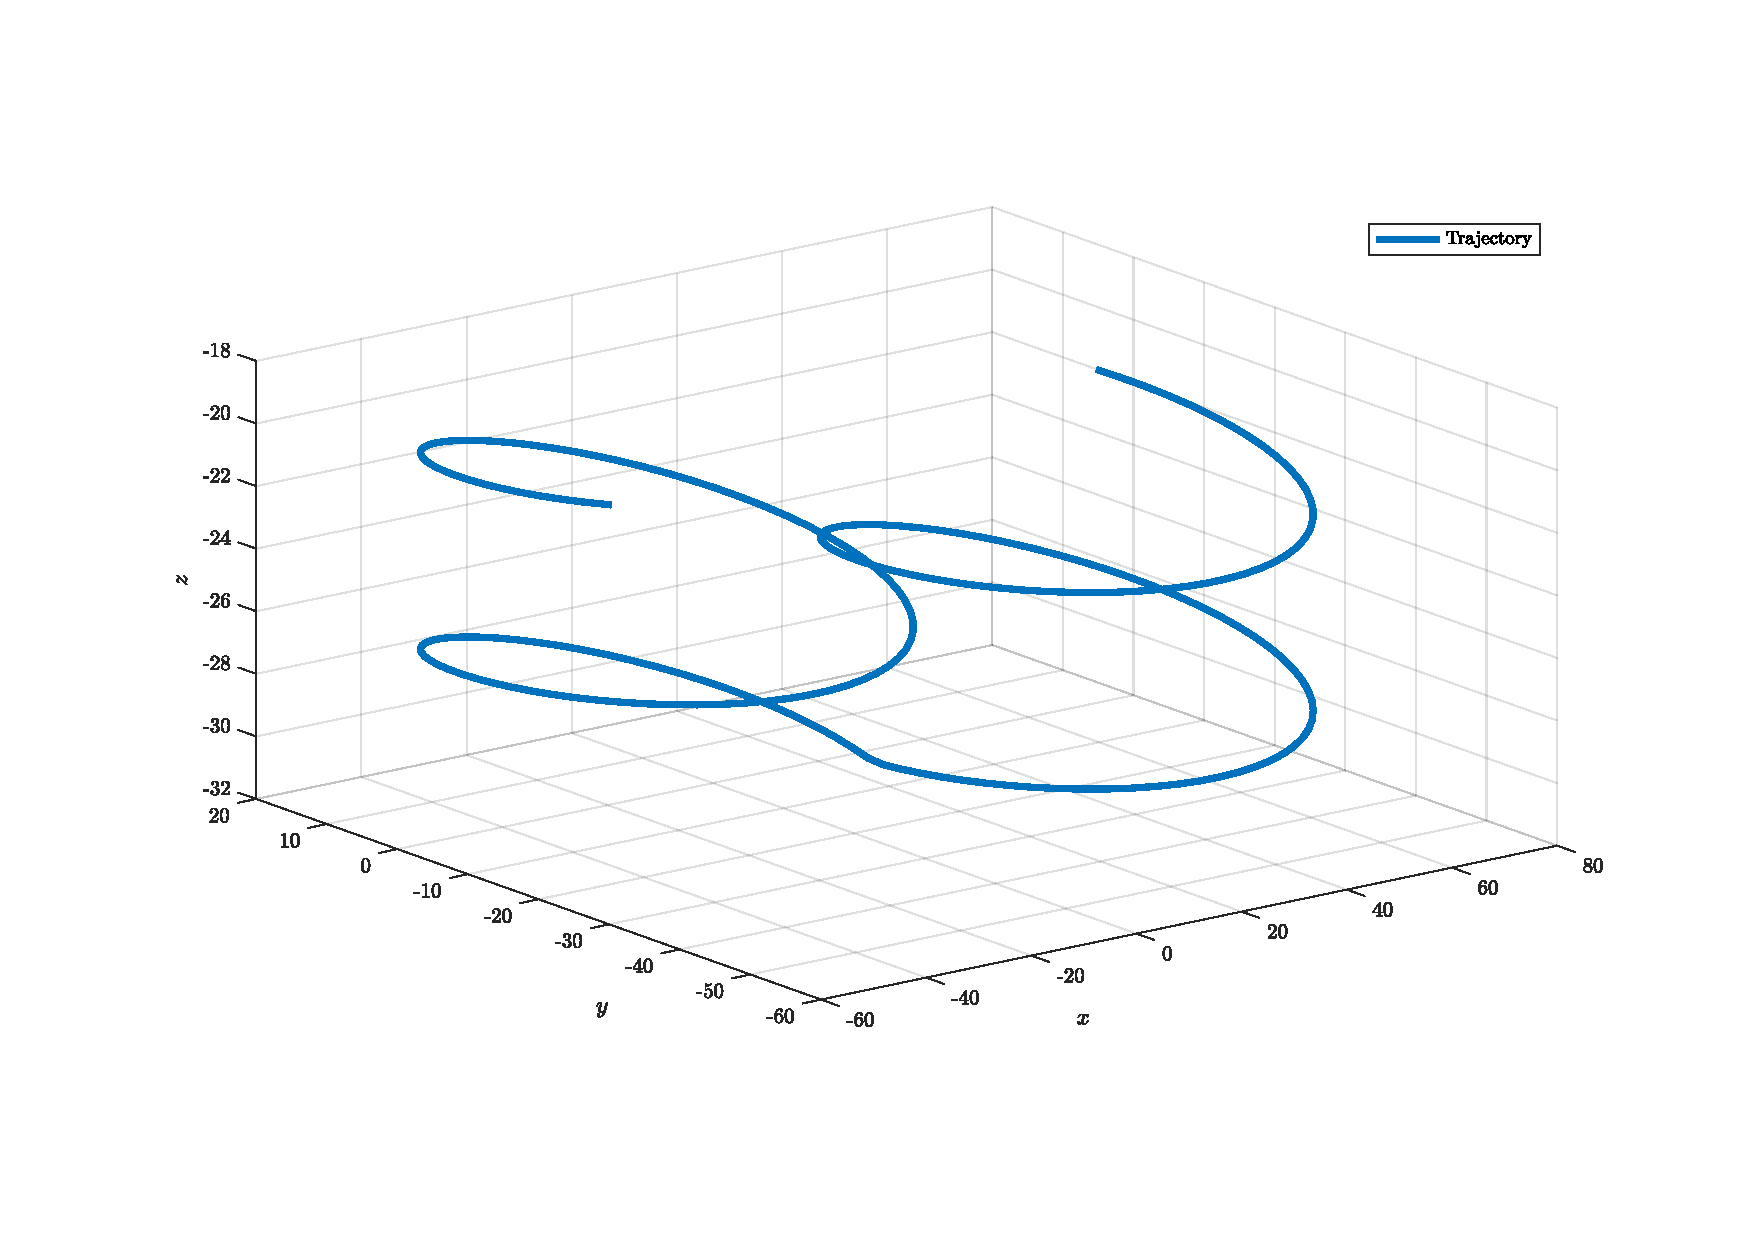
\includegraphics[width=\textwidth]{Tikz/Trajectory.tikz}			
	\caption[Simulated three-dimensional trajectory.]{Simulated three-dimensional trajectory with the start point in the upper left and the end point in the upper right hand corner.}		
	\label{fig:trajectory}			
\end{figure}

\begin{figure}
	\centering
	\setlength\figureheight{0.4\textheight} 	
	\setlength\figurewidth{0.9\textwidth}		
	\tikzsetnextfilename{Trajectory_kidnapping}		
	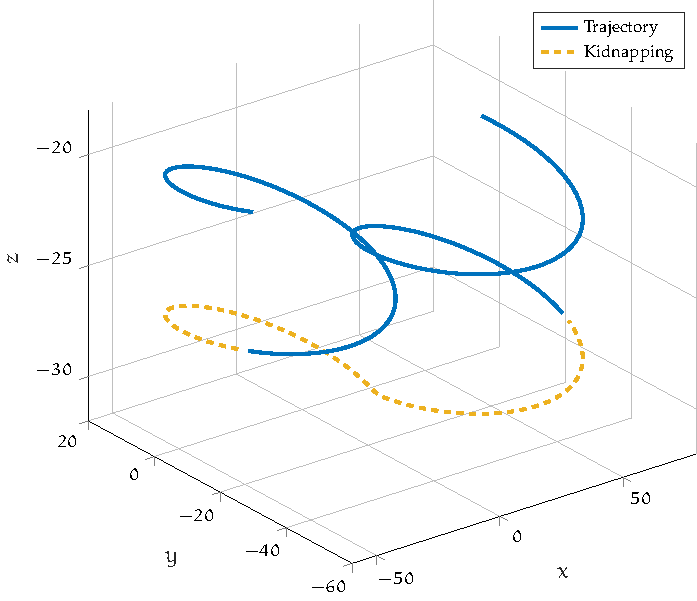
\includegraphics[width=\textwidth]{Tikz/Trajectory_kidnapping.tikz}			
	\caption[Simulated three-dimensional trajectory depicting kidnapping.]{Simulated three-dimensional trajectory with the start point in the upper left and the end point in the upper right hand corner. The part of the trajectory that is skipped through kidnapping is depicted as a yellow dashed line.}		
	\label{fig:trajectory_kidnapping}			
\end{figure}


The simulations were carried out with two, four, and nine distinguishable landmarks, respectively, in order to test the performance of the filters with ambiguous measurement data. In each of the three scenarios, the landmarks were placed in a grid above the seafloor, located about 250 metres deep. The individual position of each landmark was chosen randomly with a standard deviation of 10 metres. Figures \ref{fig:trajectory_4_with_2_landmarks}, \ref{fig:trajectory_4_with_4_landmarks}, and \ref{fig:trajectory_4_with_9_landmarks} show the trajectory in relation with the two, four, and nine landmarks, respectively. The positions of the landmarks are given in Tables \ref{tab:2landmarks}, \ref{tab:4landmarks}, and \ref{tab:9landmarks} for the respective scenario.


\begin{figure}
	\centering
	\setlength\figureheight{0.4\textheight} 	
	\setlength\figurewidth{0.9\textwidth}		
	\tikzsetnextfilename{Trajectory_4_with_2_landmarks}		
	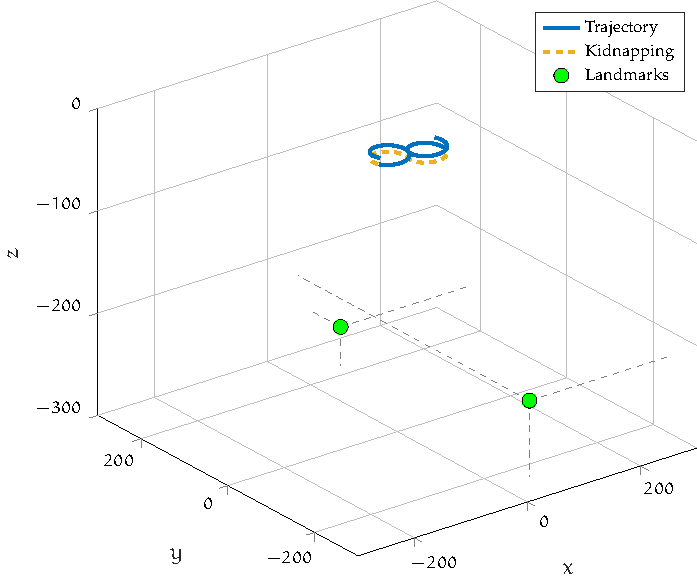
\includegraphics[width=\textwidth]{Tikz/Trajectory_4_with_2_landmarks.tikz}			
	\caption{Three-dimensional trajectory in relation with the two landmarks spread over the seabed in Scenario 1.}		
	\label{fig:trajectory_4_with_2_landmarks}			
\end{figure}
  
 \begin{figure}
	\centering
	\setlength\figureheight{0.4\textheight} 	
	\setlength\figurewidth{0.9\textwidth}		
	\tikzsetnextfilename{Trajectory_4_with_4_landmarks}		
	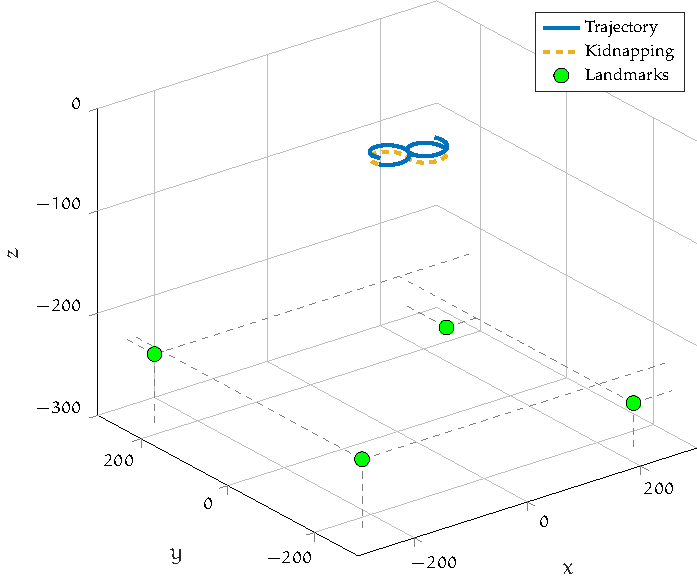
\includegraphics[width=\textwidth]{Tikz/Trajectory_4_with_4_landmarks.tikz}			
	\caption{Three-dimensional trajectory in relation with the four landmarks spread over the seabed in Scenario 2.}		
	\label{fig:trajectory_4_with_4_landmarks}			
\end{figure} 

 \begin{figure}
	\centering
	\setlength\figureheight{0.4\textheight} 	
	\setlength\figurewidth{0.9\textwidth}		
	\tikzsetnextfilename{Trajectory_4_with_9_landmarks}		
	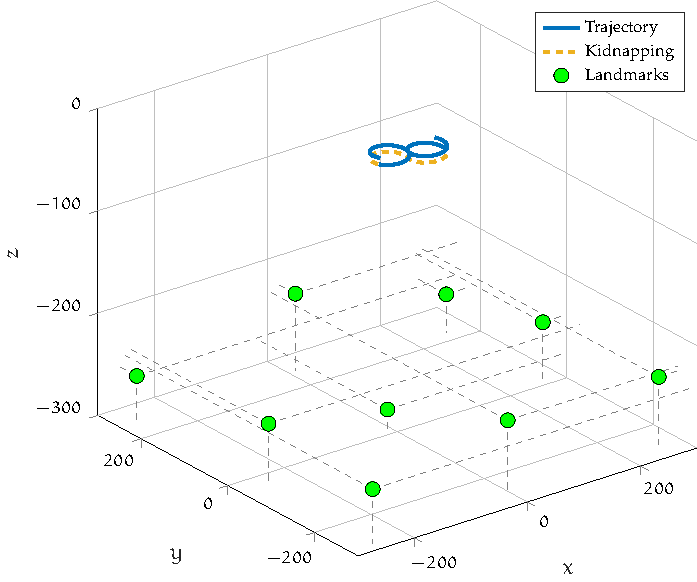
\includegraphics[width=\textwidth]{Tikz/Trajectory_4_with_9_landmarks.tikz}			
	\caption{Three-dimensional trajectory in relation with the nine landmarks spread over the seabed in Scenario 3.}		
	\label{fig:trajectory_4_with_9_landmarks}			
\end{figure} 
  
\begin{table*}\centering
\ra{1.3}
\begin{tabular}{@{}crrr@{}}\toprule
Landmark & $x$ in m & $y$ in m & $z$ in m \\
\midrule 
$1$ & $54.212$ & $-234.051$ & $-225.619$ \\               
$2$ & $72.673$ & $225.574$ & $-262.043$ \\    
\bottomrule
\end{tabular}
\caption{Positions of the landmarks in Scenario 1.}
\label{tab:2landmarks}
\end{table*}

\begin{table*}\centering
\ra{1.3}
\begin{tabular}{@{}crrr@{}}\toprule
Landmark & $x$ in m & $y$ in m & $z$ in m \\
\midrule 
$1$ & $-236.365$ & $-226.664$ & $-233.550$ \\             
$2$ & $231.643$ & $-242.535$ & $-257.183$ \\              
$3$ & $-255.960$ & $226.613$ & $-231.048$ \\              
$4$ & $247.786$ & $209.724$ & $-289.594$ \\ 
\bottomrule
\end{tabular}
\caption{Positions of the landmarks in Scenario 2.}
\label{tab:4landmarks}
\end{table*}

\begin{table*}\centering
\ra{1.3}
\begin{tabular}{@{}crrr@{}}\toprule
Landmark & $x$ in m & $y$ in m & $z$ in m \\
\midrule 
$1$ & $-258.443$ & $-279.902$ & $-246.641$ \\             
$2$ & $-1.464$ & $-256.392$ & $-229.858$ \\               
$3$ & $265.583$ & $-256.648$ & $-234.381$ \\              
$4$ & $-250.721$ & $-29.613$ & $-241.389$ \\              
$5$ & $-10.034$ & $9.951$ & $-278.862$ \\                 
$6$ & $259.375$ & $2.562$ & $-239.162$ \\                 
$7$ & $-267.623$ & $252.185$ & $-256.285$ \\              
$8$ & $12.539$ & $251.370$ & $-224.841$ \\                
$9$ & $259.698$ & $225.658$ & $-263.047$ \\    
\bottomrule
\end{tabular}
\caption{Positions of the landmarks in Scenario 3.}
\label{tab:9landmarks}
\end{table*}


\section{Performance Measures}\label{performance_measures}

The performance of the algorithms was measured computing the error $e_k$ at time step $k$ as the Euclidean distance between the estimated position $\hat{\bm{x}}_k = [\hat{x}_k, \hat{y}_k, \hat{z}_k]$ and the true position $\bm{x}_k = [x_k, y_k, z_k]$ computed by the simulator,

\begin{equation}\label{eq:lateration}
  e_k = \sqrt{(\hat{x}_k - x_k)^2 + (\hat{y}_k - y_k)^2 + (\hat{z} - z_k)^2}\,.
\end{equation}

\noindent
Given the entire sequence of estimated states $\hat{\bm{X}}_{n_s} = \{\hat{\bm{x}}_k\}^{n_s}_{k = 1}$, the root-mean-square error $\operatorname{RMSE}\big(\hat{\bm{X}}_{n_s}\big)$ is given by

\begin{equation}
  \operatorname{RMSE}\big(\hat{\bm{X}}_{n_s}\big) = \sqrt{\frac{1}{{n_s}} \sum_{k=1}^{n_s} e_k^2} \,.
\end{equation}

\noindent
In addition to the RMSE, the initial error $e_1$ was assessed. The experiments were carried out with 100000 particles for the \texttt{PF}, \texttt{PFC}, and \texttt{PFS} and 1000 particles for the \texttt{UPF}, \texttt{UPFC}, \texttt{UPFS}. In order to obtain representative results, each of the six filters was applied to the respective estimation task at hand in a hundred runs.

% as well as the time the filters took for convergence. The filter was considered to have converged when the estimation error went below one metre for the first time after the start of the estimation process or after kidnapping. 


\section{Results}\label{sec:results}

In the following, the results of the experiments described above are presented. For each of the three scenarios there are six figures, three for the respective scenario with kidnapping, and three without kidnapping. Each of the groups of three figures consists of a box plot of the estimation error distribution, a plot of the mean error sequence vs. time, and a magnified plot of the mean error sequence vs. time depicting the interesting interval with a width of 40 seconds. That is, the first 40 seconds when solving the wake-up robot problem and the 10 seconds before plus the 30 seconds after kidnapping, when solving the kidnapped robot problem. The same set of figures is presented in the appendix for 10 times fewer particles, respectively.

On each box of a box plot, the central mark indicates the median and the bottom and top edges of the box indicate the 25th and 75th percentiles, respectively. The whiskers extend to the most extreme data points not considered outliers, and the outliers are plotted individually using a red `$+$' symbol. Points are drawn as outliers if they are greater than $Q_{25} + l (Q_{75} – Q_{25})$ or less than $Q_{25} - l (Q_{75} – Q_{25})$, where $l$ is the maximum whisker length corresponding to approximately $\pm 2.7 \sigma$ and 99.3 percent coverage if the data are normally distributed.

Plots of the individual runs including the estimated trajectory in relation with the reference trajectory, the number of particles that received an importance weight of zero, and \texttt{.mat}-files containing the estimation results, with and without kidnapping, respectively, can be found on GitHub \cite{codeGithub}. In addition to that, all exact results of the individual runs and of the entire experiments, including the time of convergence and the root-mean-squared errors, can be found in the log files provided. 

\pagebreak

\subsection{Results with 2 Landmarks}

Figures \ref{fig:2018-09-30-12-09-00-results-figure-1}\,-\,\ref{fig:2018-09-30-12-09-00-results-figure-7} depicting the estimation results for Scenario 1.

\paragraph{}
%% 2 Landmarks

% 10000 / 1000

\begin{figure}[h!]
	\centering
	\setlength\figureheight{0.8\textheight} 	
	\setlength\figurewidth{1.0\textwidth}		
	\tikzsetnextfilename{2018-09-30-12-09-00-results-figure-1}		
	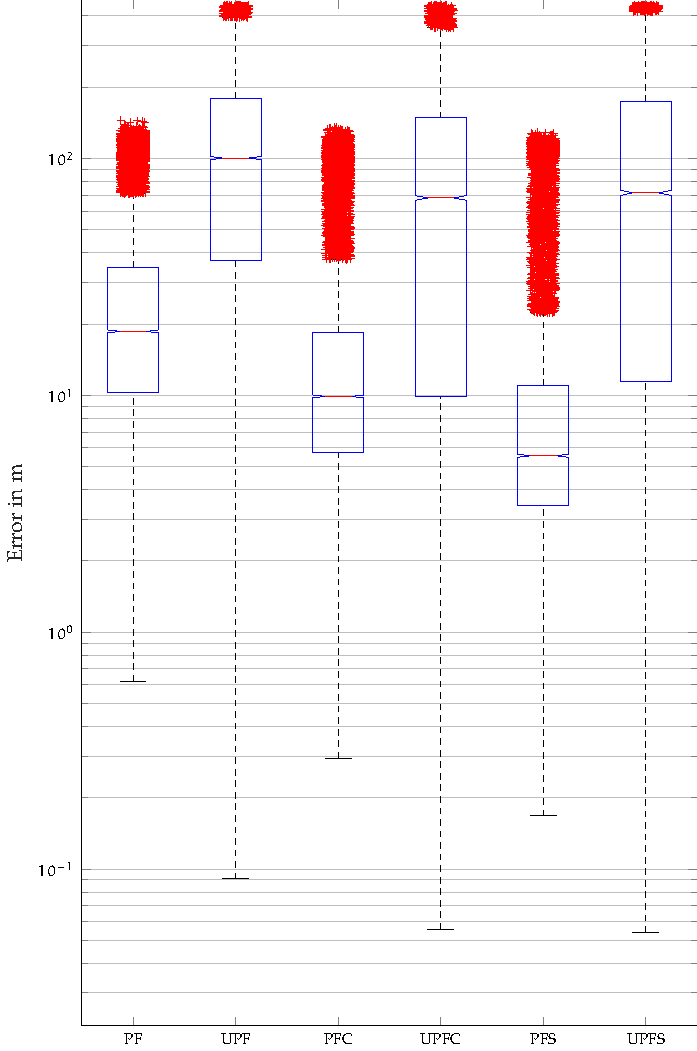
\includegraphics[width=\textwidth]{Tikz/Results/2018-09-30-12-09-00-results-figure-1.tikz}			
	\caption[Box plot of the estimation errors in Scenario 1. \texttt{PF}, \texttt{PFC}, \texttt{PFS}: 10000 particles. \texttt{UPF}, \texttt{UPFC}, \texttt{UPFS}: 1000 particles.]{Box plot of the estimation errors in Scenario 1 (logarithmic scale). \texttt{PF}, \texttt{PFC}, \texttt{PFS}: 10000 particles. \texttt{UPF}, \texttt{UPFC}, \texttt{UPFS}: 1000 particles.}
	\label{fig:2018-09-30-12-09-00-results-figure-1}			
\end{figure}

\begin{figure}
	\centering
	\setlength\figureheight{1.0\textwidth} 	
	\setlength\figurewidth{0.9\textheight}		
	\tikzsetnextfilename{2018-09-30-12-09-00-results-figure-5}		
	\rotatebox{90}{
	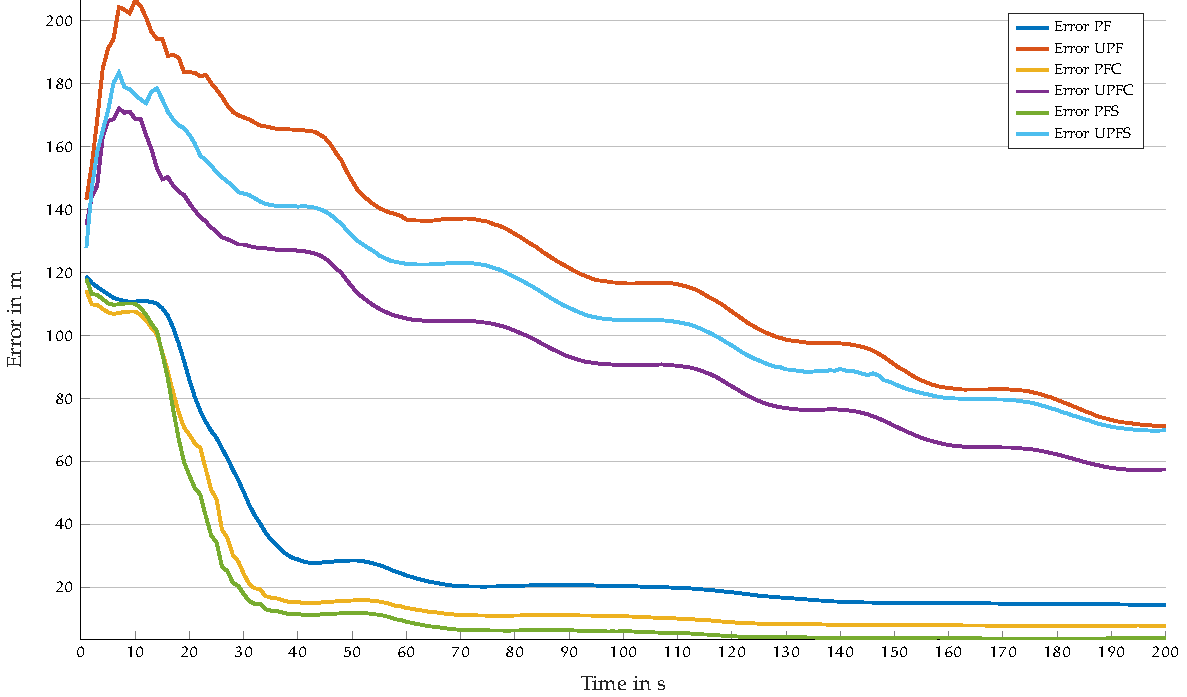
\includegraphics[height=1.0\textwidth]{Tikz/Results/2018-09-30-12-09-00-results-figure-5.tikz}}	
	\caption[Mean estimation error over time in Scenario 1. \texttt{PF}, \texttt{PFC}, \texttt{PFS}: 10000 particles. \texttt{UPF}, \texttt{UPFC}, \texttt{UPFS}: 1000 particles.]{Mean estimation error over time in Scenario 1. \texttt{PF}, \texttt{PFC}, \texttt{PFS}: 10000 particles. \texttt{UPF}, \texttt{UPFC}, \texttt{UPFS}: 1000 particles.}
	\label{fig:2018-09-30-12-09-00-results-figure-5}			
\end{figure}

\begin{figure}
	\centering
	\setlength\figureheight{1.0\textwidth} 	
	\setlength\figurewidth{0.9\textheight}		
	\tikzsetnextfilename{2018-09-30-12-09-00-results-figure-7}		
	\rotatebox{90}{
	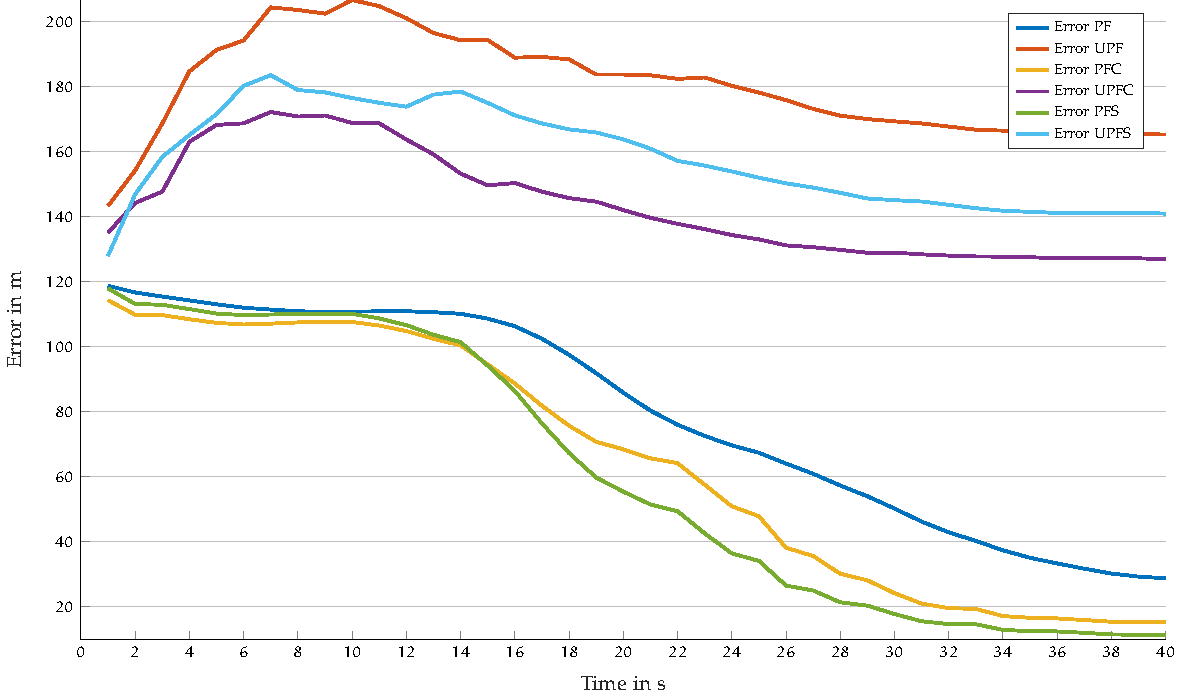
\includegraphics[height=1.0\textwidth]{Tikz/Results/2018-09-30-12-09-00-results-figure-7.tikz}}			
	\caption[First 40 seconds of the mean estimation error over time in Scenario 1. \texttt{PF}, \texttt{PFC}, \texttt{PFS}: 10000 particles. \texttt{UPF}, \texttt{UPFC}, \texttt{UPFS}: 1000 particles.]{First 40 seconds of the mean estimation error over time in Scenario 1. \texttt{PF}, \texttt{PFC}, \texttt{PFS}: 10000 particles. \texttt{UPF}, \texttt{UPFC}, \texttt{UPFS}: 1000 particles.}
	\label{fig:2018-09-30-12-09-00-results-figure-7}			
\end{figure}


\subsection{Results with 2 Landmarks and Kidnapping}

Figures \ref{fig:2018-10-04-15-13-55-results-figure-1}\,-\,\ref{fig:2018-10-04-15-13-55-results-figure-8} depicting the estimation results for Scenario 1 with kidnapping.

\paragraph{}
%% 2 Landmarks kidnapping

% 10000 / 1000

\begin{figure}[h!]
	\centering
	\setlength\figureheight{0.8\textheight} 	
	\setlength\figurewidth{1.0\textwidth}		
	\tikzsetnextfilename{2018-10-04-15-13-55-results-figure-1}		
	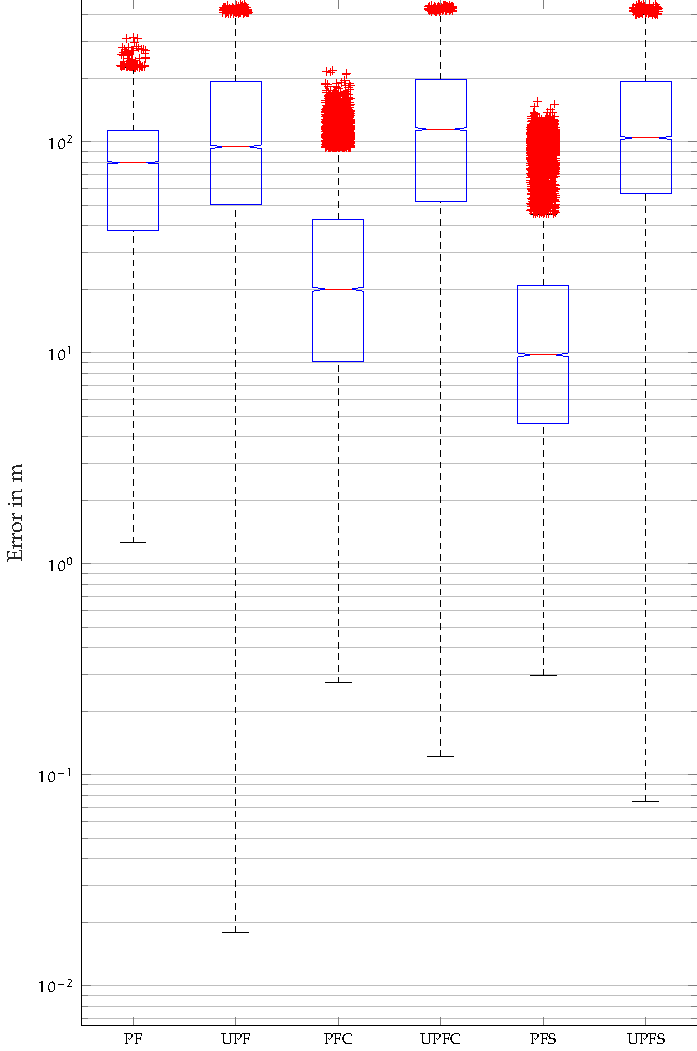
\includegraphics[width=\textwidth]{Tikz/Results/2018-10-04-15-13-55-results-figure-1.tikz}			
	\caption[Box plot of the estimation errors in Scenario 1 with kidnapping. \texttt{PF}, \texttt{PFC}, \texttt{PFS}: 10000 particles. \texttt{UPF}, \texttt{UPFC}, \texttt{UPFS}: 1000 particles.]{Box plot of the estimation errors in Scenario 1 with kidnapping (logarithmic scale). \texttt{PF}, \texttt{PFC}, \texttt{PFS}: 10000 particles. \texttt{UPF}, \texttt{UPFC}, \texttt{UPFS}: 1000 particles.}
	\label{fig:2018-10-04-15-13-55-results-figure-1}			
\end{figure}

\begin{figure}
	\centering
	\setlength\figureheight{1.0\textwidth} 	
	\setlength\figurewidth{0.9\textheight}		
	\tikzsetnextfilename{2018-10-04-15-13-55-results-figure-6}		
	\rotatebox{90}{
	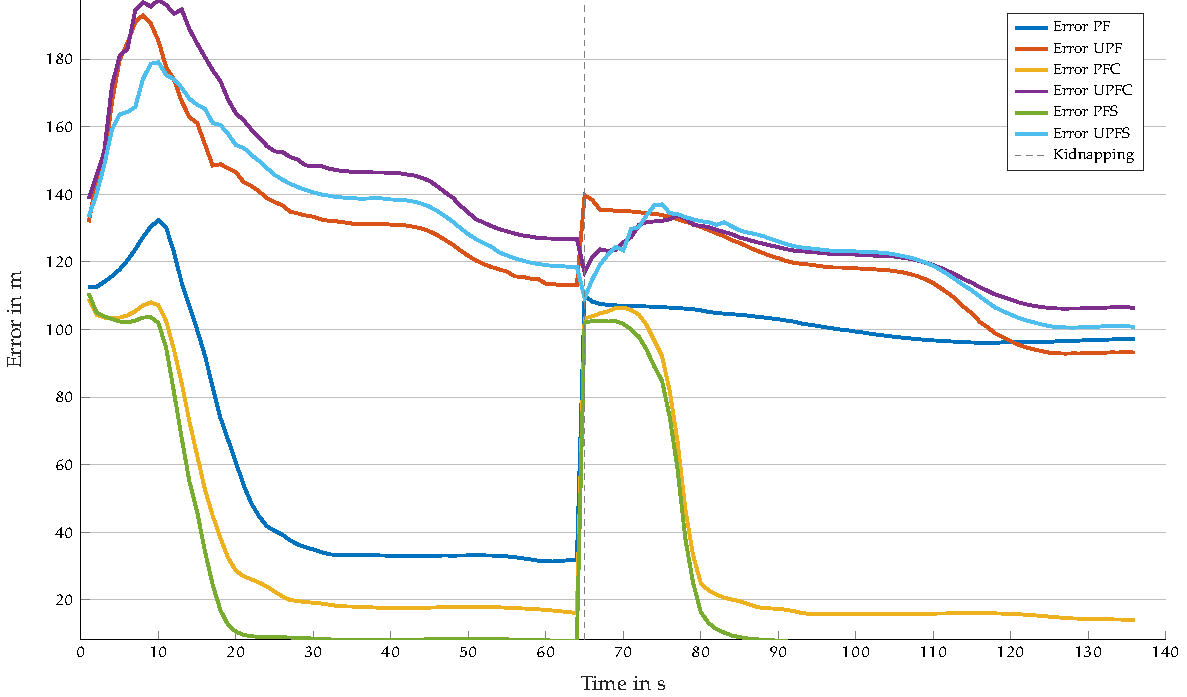
\includegraphics[height=1.0\textwidth]{Tikz/Results/2018-10-04-15-13-55-results-figure-6.tikz}}			
	\caption[Mean estimation error over time in Scenario 1 with kidnapping. \texttt{PF}, \texttt{PFC}, \texttt{PFS}: 10000 particles. \texttt{UPF}, \texttt{UPFC}, \texttt{UPFS}: 1000 particles.]{Mean estimation error over time in Scenario 1 with kidnapping. \texttt{PF}, \texttt{PFC}, \texttt{PFS}: 10000 particles. \texttt{UPF}, \texttt{UPFC}, \texttt{UPFS}: 1000 particles.}
	\label{fig:2018-10-04-15-13-55-results-figure-6}			
\end{figure}

\begin{figure}
	\centering
	\setlength\figureheight{1.0\textwidth} 	
	\setlength\figurewidth{0.9\textheight}		
	\tikzsetnextfilename{2018-10-04-15-13-55-results-figure-8}		
	\rotatebox{90}{
	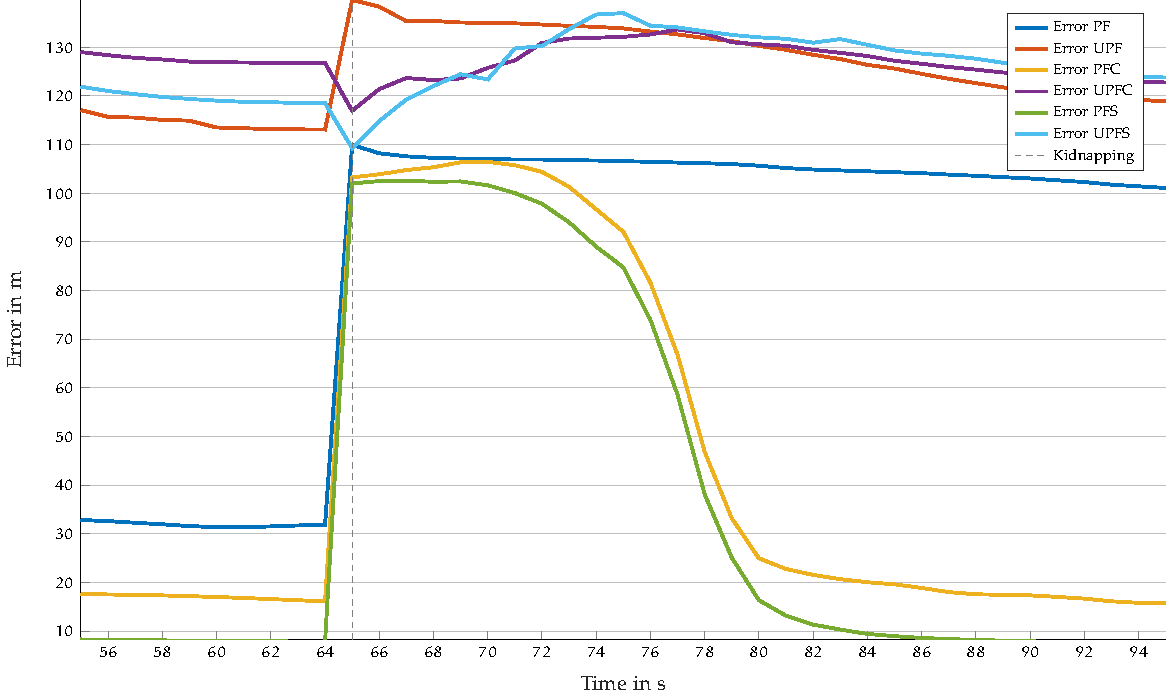
\includegraphics[height=1.0\textwidth]{Tikz/Results/2018-10-04-15-13-55-results-figure-8.tikz}}			
	\caption[First 30 seconds of the mean estimation error over time after kidnapping in Scenario 1. \texttt{PF}, \texttt{PFC}, \texttt{PFS}: 10000 particles. \texttt{UPF}, \texttt{UPFC}, \texttt{UPFS}: 1000 particles.]{First 30 seconds of the mean estimation error over time after kidnapping in Scenario 1. \texttt{PF}, \texttt{PFC}, \texttt{PFS}: 10000 particles. \texttt{UPF}, \texttt{UPFC}, \texttt{UPFS}: 1000 particles.}	
	\label{fig:2018-10-04-15-13-55-results-figure-8}			
\end{figure}


\subsection{Results with 4 Landmarks}

Figures \ref{fig:2018-09-24-11-26-33-results-figure-1}\,-\,\ref{fig:2018-09-24-11-26-33-results-figure-7} depicting the estimation results for Scenario 2.

\paragraph{}
%% 4 Landmarks

% 10000 / 100

\begin{figure}[h!]
	\centering
	\setlength\figureheight{0.8\textheight} 	
	\setlength\figurewidth{1.0\textwidth}		
	\tikzsetnextfilename{2018-09-24-11-26-33-results-figure-1}		
	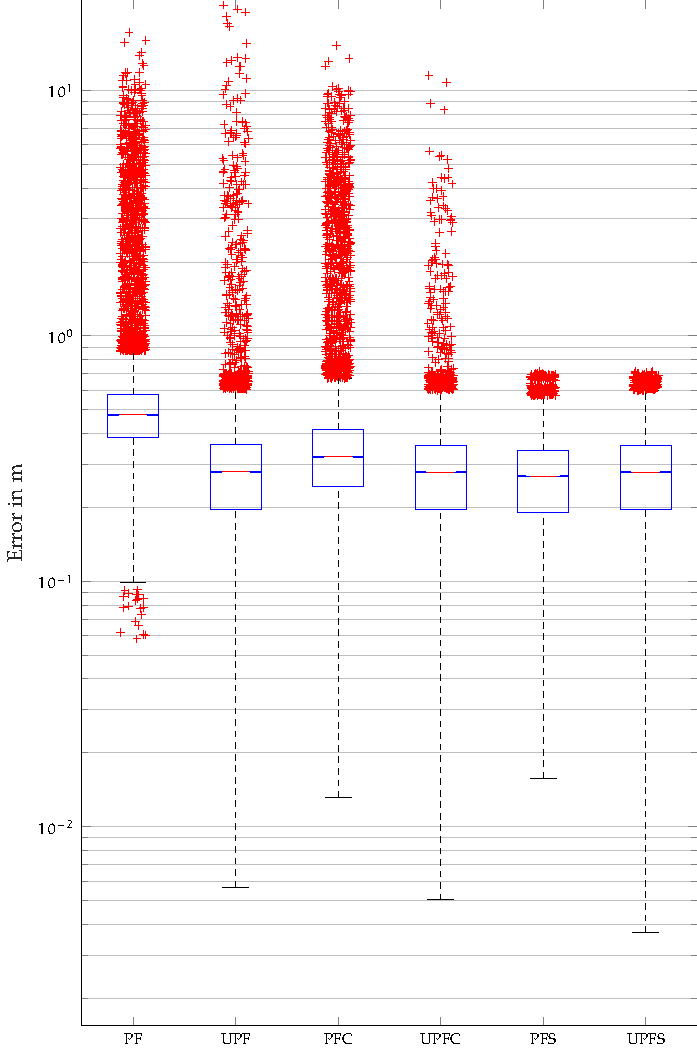
\includegraphics[width=\textwidth]{Tikz/Results/2018-09-24-11-26-33-results-figure-1.tikz}			
	\caption[Box plot of the estimation errors in Scenario 2. \texttt{PF}, \texttt{PFC}, \texttt{PFS}: 10000 particles. \texttt{UPF}, \texttt{UPFC}, \texttt{UPFS}: 100 particles.]{Box plot of the estimation errors in Scenario 2 (logarithmic scale). \texttt{PF}, \texttt{PFC}, \texttt{PFS}: 10000 particles. \texttt{UPF}, \texttt{UPFC}, \texttt{UPFS}: 100 particles.}
	\label{fig:2018-09-24-11-26-33-results-figure-1}			
\end{figure}

\begin{figure}
	\centering
	\setlength\figureheight{1.0\textwidth} 	
	\setlength\figurewidth{0.9\textheight}		
	\tikzsetnextfilename{2018-09-24-11-26-33-results-figure-5}		
	\rotatebox{90}{
	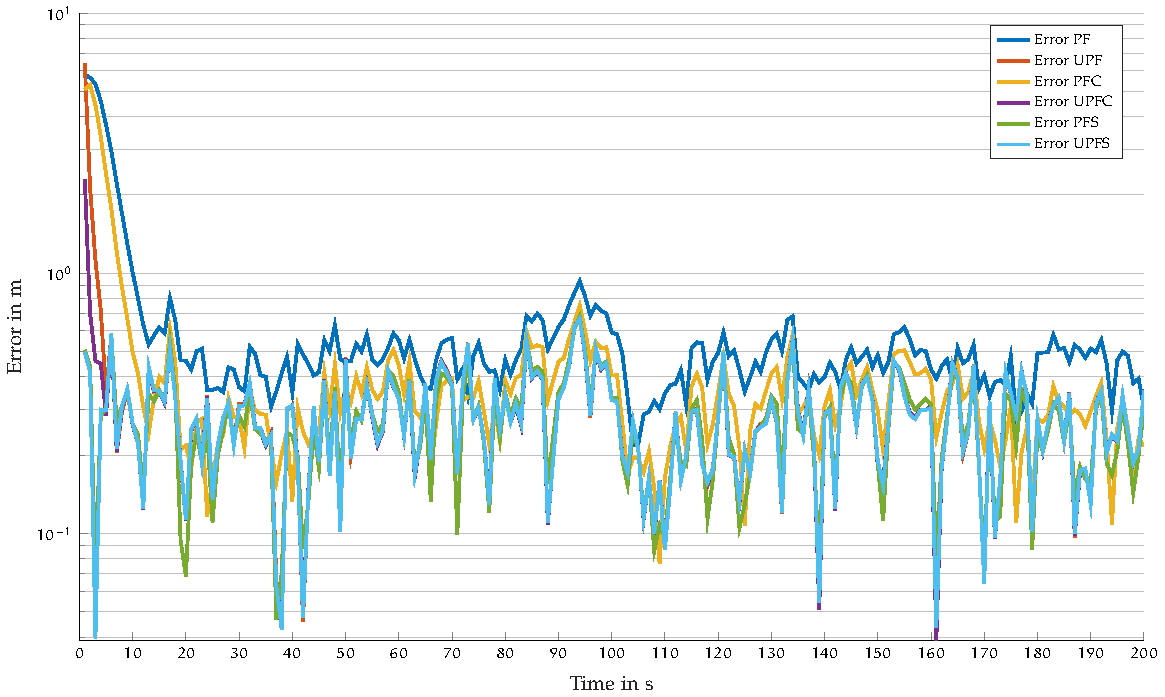
\includegraphics[height=1.0\textwidth]{Tikz/Results/2018-09-24-11-26-33-results-figure-5.tikz}}			
	\caption[Mean estimation error over time in Scenario 2. \texttt{PF}, \texttt{PFC}, \texttt{PFS}: 10000 particles. \texttt{UPF}, \texttt{UPFC}, \texttt{UPFS}: 100 particles.]{Mean estimation error over time in Scenario 2 (logarithmic scale). \texttt{PF}, \texttt{PFC}, \texttt{PFS}: 10000 particles. \texttt{UPF}, \texttt{UPFC}, \texttt{UPFS}: 100 particles.}
	\label{fig:2018-09-24-11-26-33-results-figure-5}			
\end{figure}

\begin{figure}
	\centering
	\setlength\figureheight{1.0\textwidth} 	
	\setlength\figurewidth{0.9\textheight}		
	\tikzsetnextfilename{2018-09-24-11-26-33-results-figure-7}		
	\rotatebox{90}{
	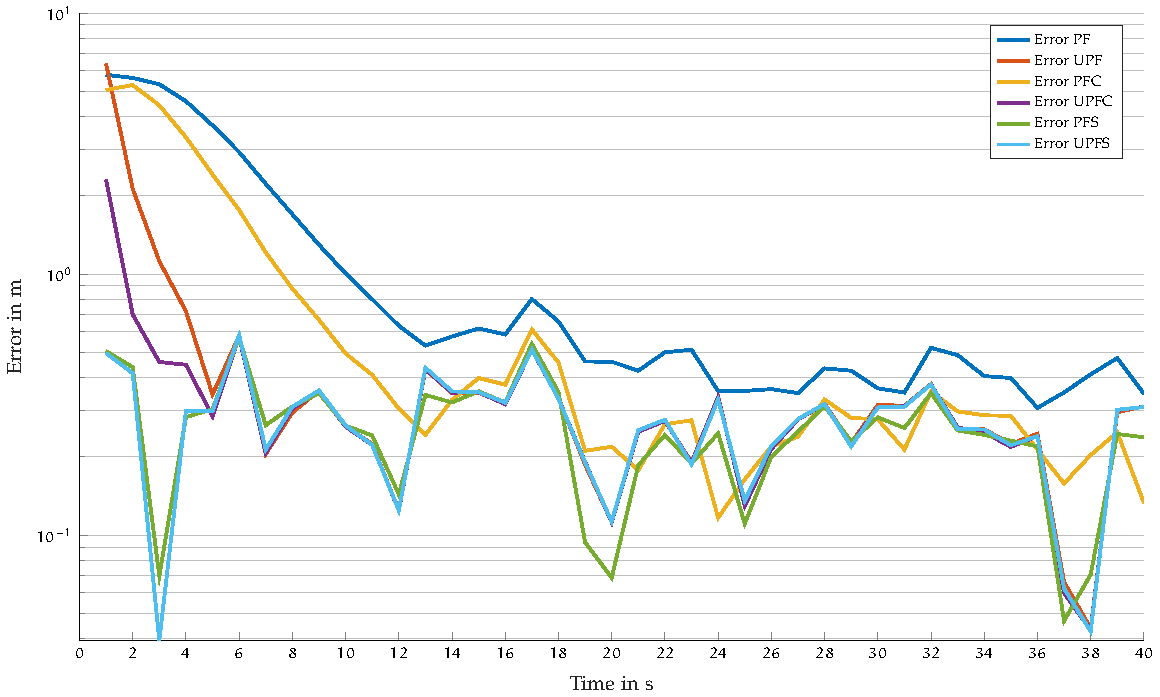
\includegraphics[height=1.0\textwidth]{Tikz/Results/2018-09-24-11-26-33-results-figure-7.tikz}}			
	\caption[First 40 seconds of the mean estimation error over time in Scenario 2. \texttt{PF}, \texttt{PFC}, \texttt{PFS}: 10000 particles. \texttt{UPF}, \texttt{UPFC}, \texttt{UPFS}: 100 particles.]{First 40 seconds of the mean estimation error over time in Scenario 2 (logarithmic scale). \texttt{PF}, \texttt{PFC}, \texttt{PFS}: 10000 particles. \texttt{UPF}, \texttt{UPFC}, \texttt{UPFS}: 100 particles.}
	\label{fig:2018-09-24-11-26-33-results-figure-7}			
\end{figure}



\subsection{Results with 4 Landmarks and Kidnapping}

Figures \ref{fig:2018-09-21-21-56-07-results-figure-1}\,-\,\ref{fig:2018-09-21-21-56-07-results-figure-8} depicting the estimation results for Scenario 2 with kidnapping.

\paragraph{}

%% 4 Landmarks kidnapping

% 10000 / 100

\begin{figure}[h!]
	\centering
	\setlength\figureheight{0.8\textheight} 	
	\setlength\figurewidth{1.0\textwidth}		
	\tikzsetnextfilename{2018-09-21-21-56-07-results-figure-1}		
	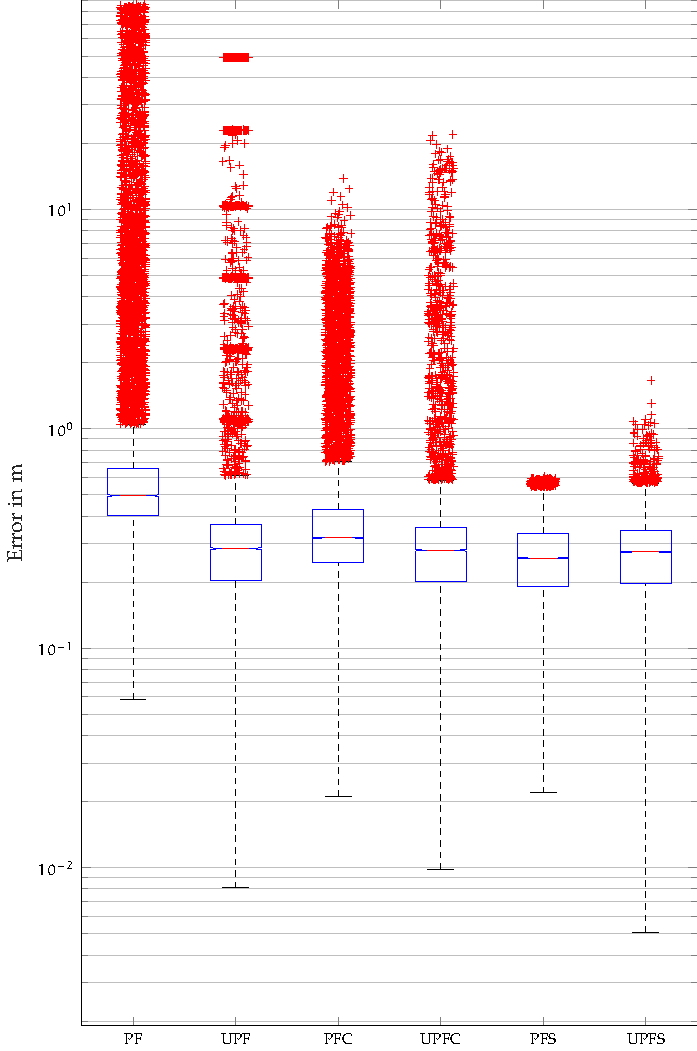
\includegraphics[width=\textwidth]{Tikz/Results/2018-09-21-21-56-07-results-figure-1.tikz}			
	\caption[Box plot of the estimation errors in Scenario 2 with kidnapping. \texttt{PF}, \texttt{PFC}, \texttt{PFS}: 10000 particles. \texttt{UPF}, \texttt{UPFC}, \texttt{UPFS}: 100 particles.]{Box plot of the estimation errors in Scenario 2 with kidnapping (logarithmic scale). \texttt{PF}, \texttt{PFC}, \texttt{PFS}: 10000 particles. \texttt{UPF}, \texttt{UPFC}, \texttt{UPFS}: 100 particles.}	
	\label{fig:2018-09-21-21-56-07-results-figure-1}			
\end{figure}

\begin{figure}
	\centering
	\setlength\figureheight{1.0\textwidth} 	
	\setlength\figurewidth{0.9\textheight}		
	\tikzsetnextfilename{2018-09-21-21-56-07-results-figure-6}		
	\rotatebox{90}{
	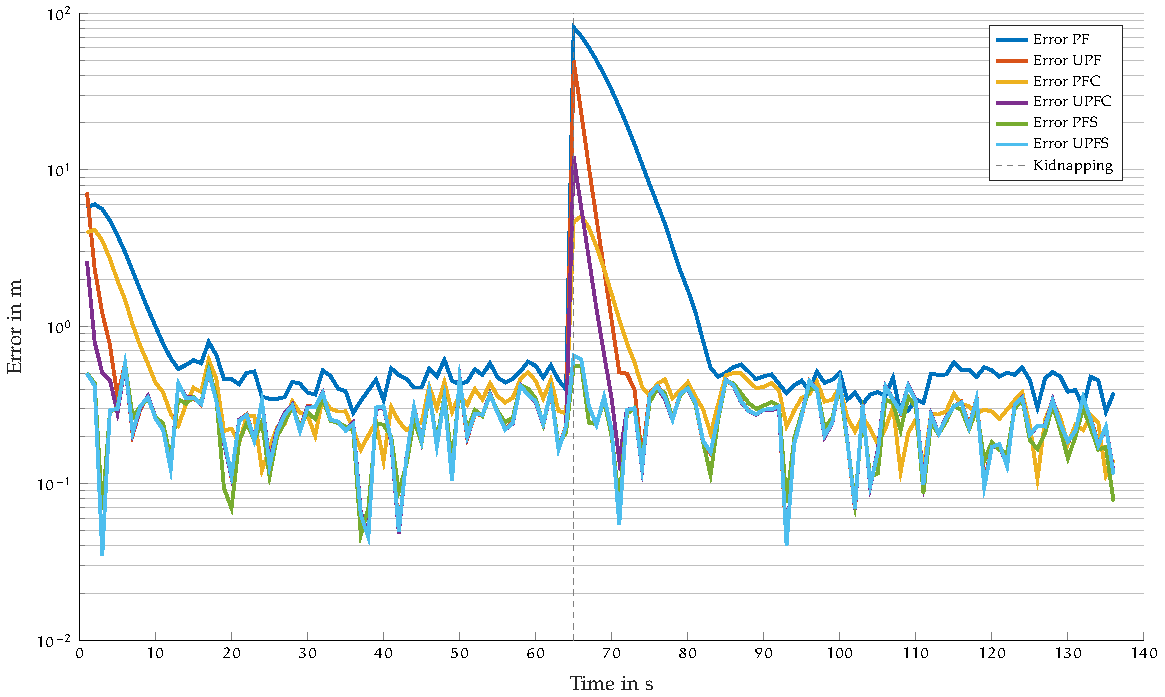
\includegraphics[height=1.0\textwidth]{Tikz/Results/2018-09-21-21-56-07-results-figure-6.tikz}}			
	\caption[Mean estimation error over time in Scenario 2 with kidnapping. \texttt{PF}, \texttt{PFC}, \texttt{PFS}: 10000 particles. \texttt{UPF}, \texttt{UPFC}, \texttt{UPFS}: 100 particles.]{Mean estimation error over time in Scenario 2 with kidnapping (logarithmic scale). \texttt{PF}, \texttt{PFC}, \texttt{PFS}: 10000 particles. \texttt{UPF}, \texttt{UPFC}, \texttt{UPFS}: 100 particles.}	
	\label{fig:2018-09-21-21-56-07-results-figure-6}			
\end{figure}

\begin{figure}
	\centering
	\setlength\figureheight{1.0\textwidth} 	
	\setlength\figurewidth{0.9\textheight}		
	\tikzsetnextfilename{2018-09-21-21-56-07-results-figure-8}		
	\rotatebox{90}{
	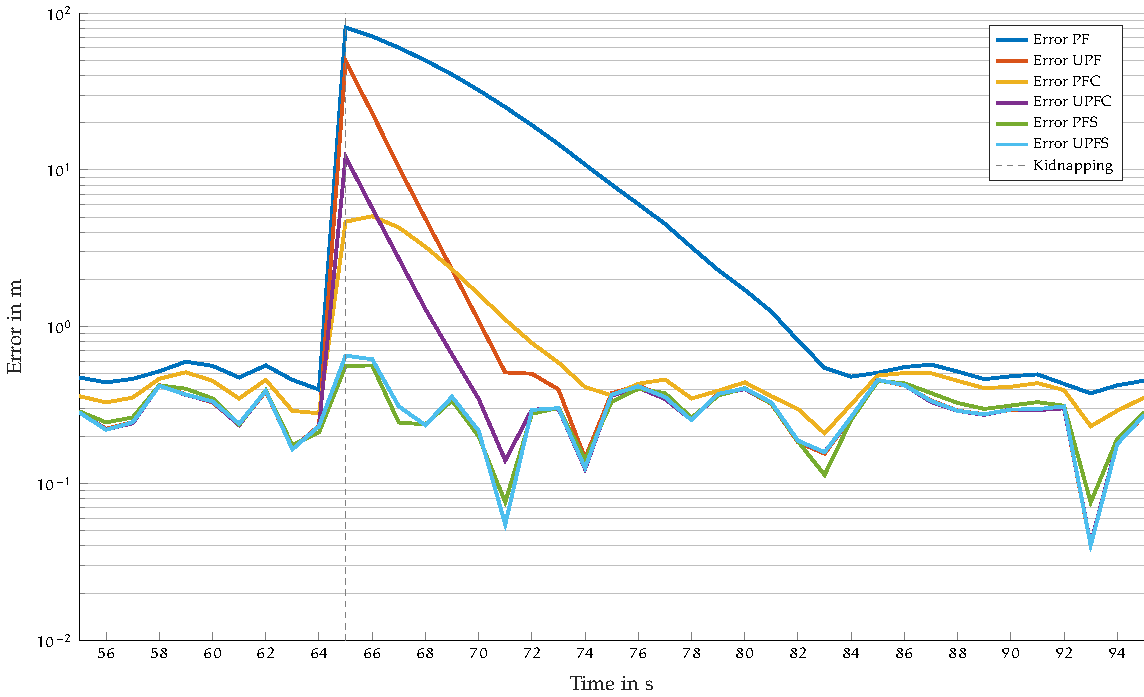
\includegraphics[height=1.0\textwidth]{Tikz/Results/2018-09-21-21-56-07-results-figure-8.tikz}}			
	\caption[First 30 seconds of the mean estimation error over time after kidnapping in Scenario 2. \texttt{PF}, \texttt{PFC}, \texttt{PFS}: 10000 particles. \texttt{UPF}, \texttt{UPFC}, \texttt{UPFS}: 100 particles.]{First 30 seconds of the mean estimation error over time after kidnapping in Scenario 2 (logarithmic scale). \texttt{PF}, \texttt{PFC}, \texttt{PFS}: 10000 particles. \texttt{UPF}, \texttt{UPFC}, \texttt{UPFS}: 100 particles.}
	\label{fig:2018-09-21-21-56-07-results-figure-8}			
\end{figure}


\subsection{Results with 9 Landmarks}

Figures \ref{fig:2018-08-30-19-17-11-results-figure-1}\,-\,\ref{fig:2018-08-30-19-17-11-results-figure-6} depicting the estimation results for Scenario 3.



%Table \ref{tab:parameters_scenario3} shows the filter parameters used for the individual filters.
%
%\begin{table*}
%\centering
%\ra{1.3}
%\begin{tabular}{@{}lrrrrrr@{}}\toprule
% & PF & UPF & PFC & UPFC & PFS & UPFS \\   
% \midrule              
%$\sigma_{v}$ in \unitfrac[]{m}{s} & $4.00$ & - & $0.80$ & - & - & - \\
%$\sigma_{YPR}$ in ° & $10.00$ & - & $2.00$ & - & - & - \\
%$\sigma_{Lik}$ in m & $15.00$ & $3.00$ & $1.50$ & $0.30$ & $1.50$ & $0.30$ \\
%$\sigma_{Trans}$ in m & - & $41.75$ & - & $20.87$ & - & $20.87$ \\
%$\sigma_{P_0}$ in m & - & $100.00$ & - & $1.00$ & - & $1.00$ \\
%$\sigma_{v_Q}$ in \unitfrac[]{m}{s} & - & $0.04$ & - & $0.02$ & - & $0.02$ \\
%$\sigma_{YPR_Q}$ in ° & - & $0.10$ & - & $0.05$ & - & $0.05$ \\
%$\sigma_{R}$ in m & - & $0.03$ & - & $0.03$ & - & $0.03$ \\    
%\bottomrule
%\end{tabular}
%\caption[Filter parameters for Scenario 3.]{Parameterisation for the six filters in Scenario 3: particle filter (PF), unscented particle filter (UPF), particle filter with contractor (PFC), unscented particle filter with contractor (UPFC), particle filter with \texttt{SIVIA} (PFS), unscented particle filter with \texttt{SIVIA} (UPFS).}
%\label{tab:parameters_scenario3}
%\end{table*}


\paragraph{}

%% 9 Landmarks

% 10000 / 100

\begin{figure}[h!]
	\centering
	\setlength\figureheight{0.8\textheight} 	
	\setlength\figurewidth{1.0\textwidth}		
	\tikzsetnextfilename{2018-08-30-19-17-11-results-figure-1}		
	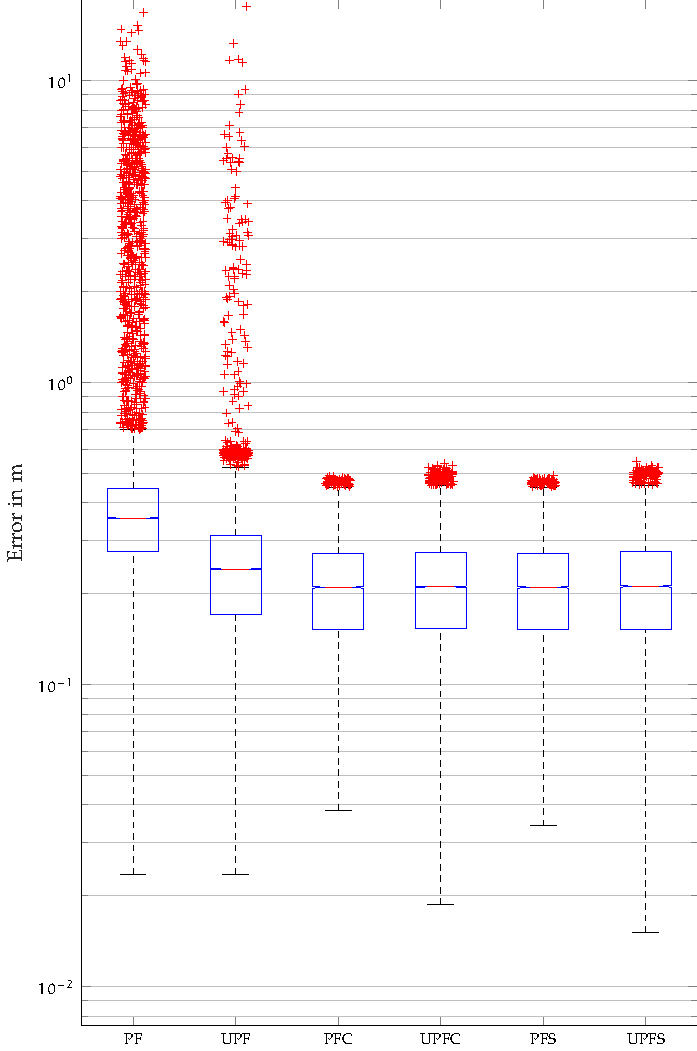
\includegraphics[width=\textwidth]{Tikz/Results/2018-08-30-19-17-11-results-figure-1.tikz}			
	\caption[Box plot of the estimation errors in Scenario 3. \texttt{PF}, \texttt{PFC}, \texttt{PFS}: 10000 particles. \texttt{UPF}, \texttt{UPFC}, \texttt{UPFS}: 100 particles.]{Box plot of the estimation errors in Scenario 3 (logarithmic scale). \texttt{PF}, \texttt{PFC}, \texttt{PFS}: 10000 particles. \texttt{UPF}, \texttt{UPFC}, \texttt{UPFS}: 100 particles.}
	\label{fig:2018-08-30-19-17-11-results-figure-1}			
\end{figure}

\begin{figure}
	\centering
	\setlength\figureheight{1.0\textwidth} 	
	\setlength\figurewidth{0.9\textheight}		
	\tikzsetnextfilename{2018-08-30-19-17-11-results-figure-4}		
	\rotatebox{90}{
	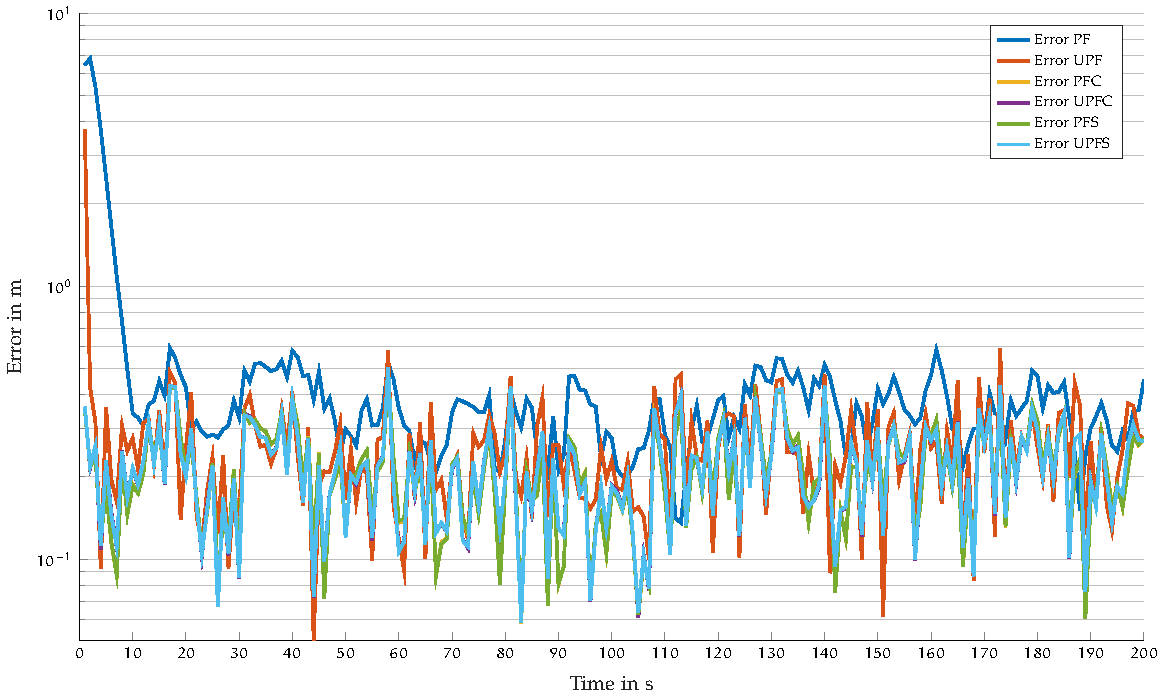
\includegraphics[height=1.0\textwidth]{Tikz/Results/2018-08-30-19-17-11-results-figure-4.tikz}}			
	\caption[Mean estimation error over time in Scenario 3. \texttt{PF}, \texttt{PFC}, \texttt{PFS}: 10000 particles. \texttt{UPF}, \texttt{UPFC}, \texttt{UPFS}: 100 particles.]{Mean estimation error over time in Scenario 3 (logarithmic scale). \texttt{PF}, \texttt{PFC}, \texttt{PFS}: 10000 particles. \texttt{UPF}, \texttt{UPFC}, \texttt{UPFS}: 100 particles.}
	\label{fig:2018-08-30-19-17-11-results-figure-4}			
\end{figure}

\begin{figure}
	\centering
	\setlength\figureheight{1.0\textwidth} 	
	\setlength\figurewidth{0.9\textheight}		
	\tikzsetnextfilename{2018-08-30-19-17-11-results-figure-6}		
	\rotatebox{90}{
	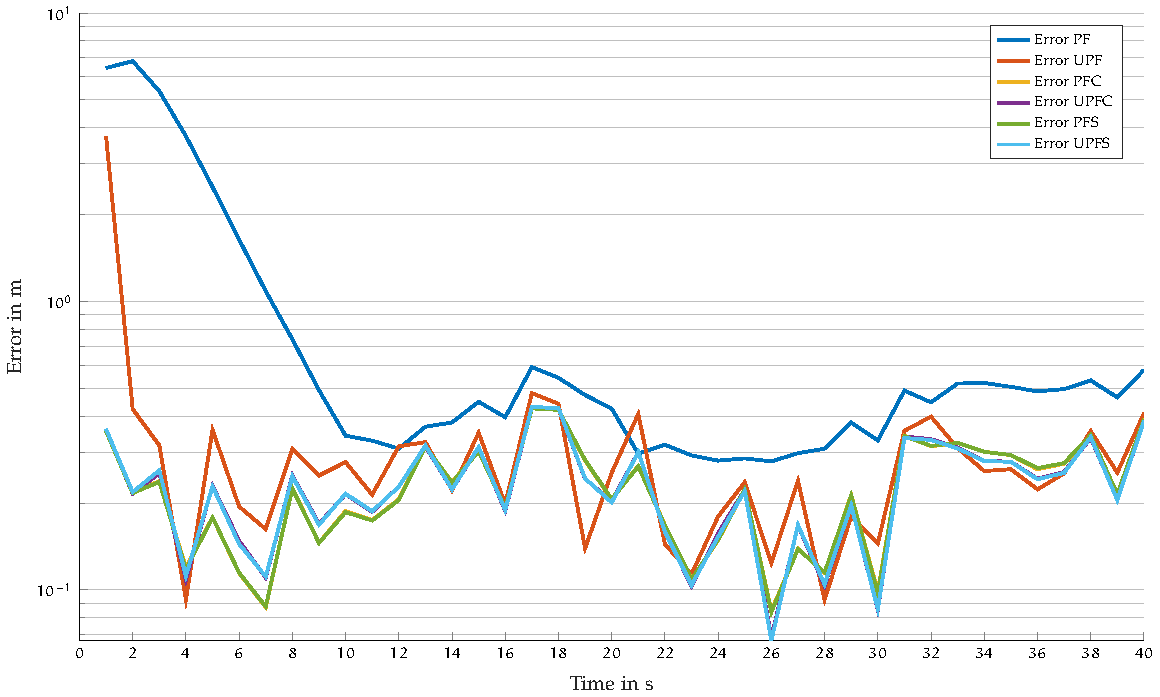
\includegraphics[height=1.0\textwidth]{Tikz/Results/2018-08-30-19-17-11-results-figure-6.tikz}}			
	\caption[First 40 seconds of the mean estimation error over time in Scenario 3. \texttt{PF}, \texttt{PFC}, \texttt{PFS}: 10000 particles. \texttt{UPF}, \texttt{UPFC}, \texttt{UPFS}: 100 particles.]{First 40 seconds of the mean estimation error over time in Scenario 3 (logarithmic scale). \texttt{PF}, \texttt{PFC}, \texttt{PFS}: 10000 particles. \texttt{UPF}, \texttt{UPFC}, \texttt{UPFS}: 100 particles.}
	\label{fig:2018-08-30-19-17-11-results-figure-6}			
\end{figure}


\subsection{Results with 9 Landmarks and Kidnapping}

Figures \ref{fig:2018-09-03-13-54-12-results-figure-1}\,-\,\ref{fig:2018-09-03-13-54-12-results-figure-6} depicting the estimation results for Scenario 3 with kidnapping.

\paragraph{}

%% 9 Landmarks kidnapping

% 10000 / 100

\begin{figure}[h!]
	\centering
	\setlength\figureheight{0.8\textheight} 	
	\setlength\figurewidth{1.0\textwidth}		
	\tikzsetnextfilename{2018-09-03-13-54-12-results-figure-1}		
	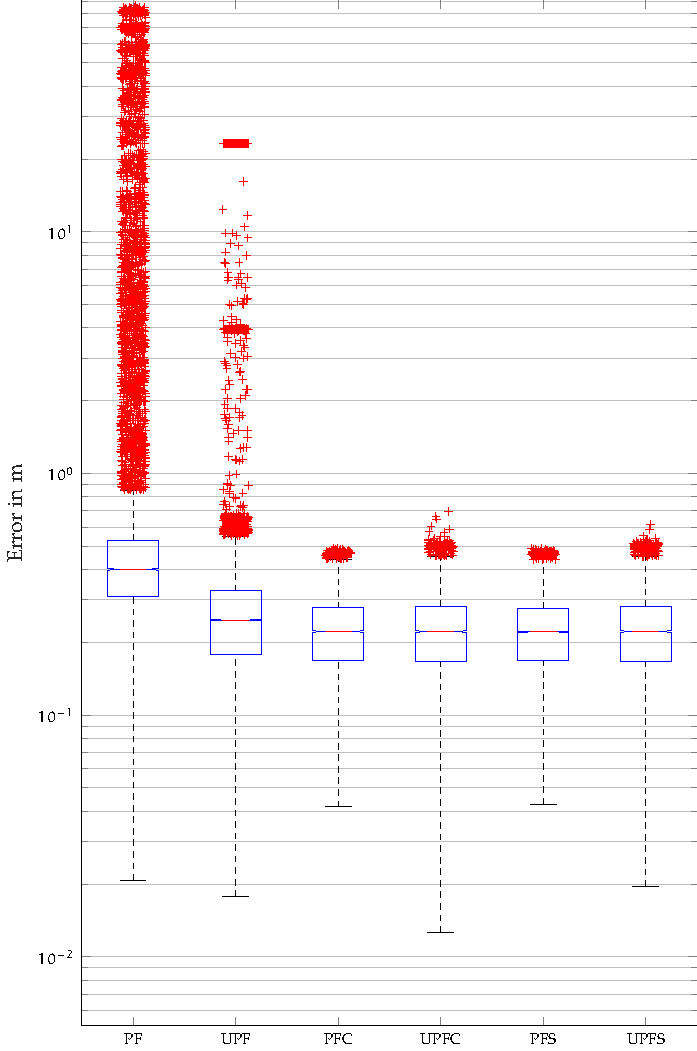
\includegraphics[width=\textwidth]{Tikz/Results/2018-09-03-13-54-12-results-figure-1.tikz}			
	\caption[Box plot of the estimation errors in Scenario 3 with kidnapping. \texttt{PF}, \texttt{PFC}, \texttt{PFS}: 10000 particles. \texttt{UPF}, \texttt{UPFC}, \texttt{UPFS}: 100 particles.]
	{Box plot of the estimation errors in Scenario 3 with kidnapping (logarithmic scale). \texttt{PF}, \texttt{PFC}, \texttt{PFS}: 10000 particles. \texttt{UPF}, \texttt{UPFC}, \texttt{UPFS}: 100 particles.}
	\label{fig:2018-09-03-13-54-12-results-figure-1}			
\end{figure}

\begin{figure}
	\centering
	\setlength\figureheight{1.0\textwidth} 	
	\setlength\figurewidth{0.9\textheight}		
	\tikzsetnextfilename{2018-09-03-13-54-12-results-figure-4}		
	\rotatebox{90}{
	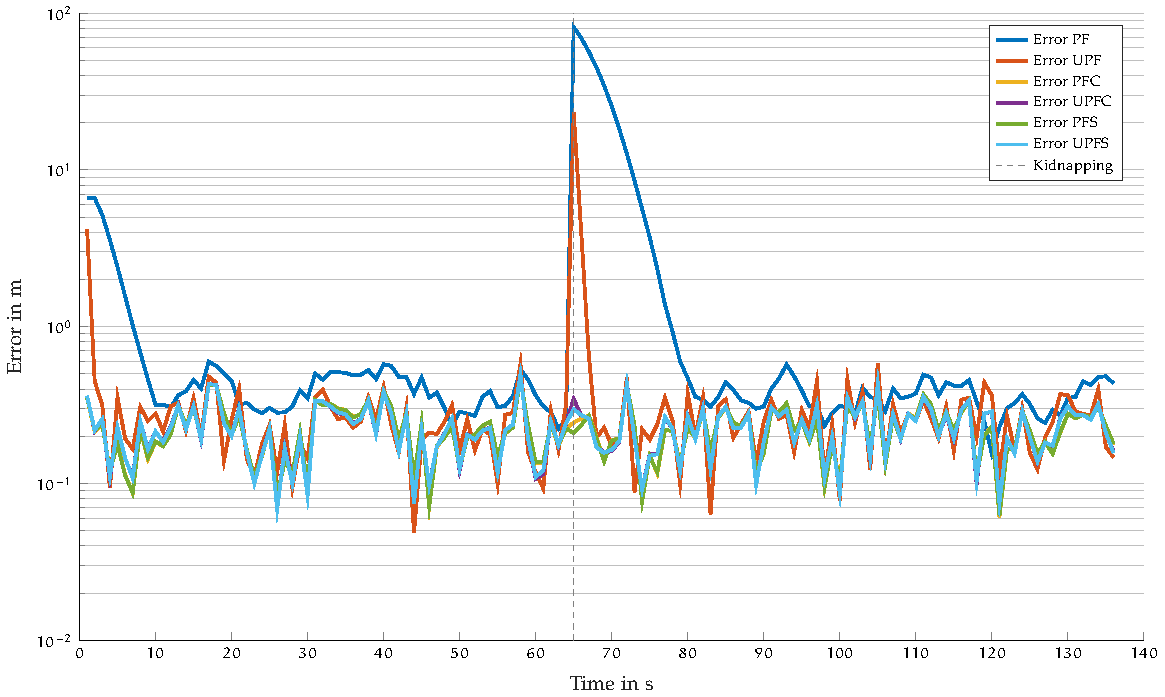
\includegraphics[height=1.0\textwidth]{Tikz/Results/2018-09-03-13-54-12-results-figure-4.tikz}}			
	\caption[Mean estimation error over time in Scenario 3 with kidnapping. \texttt{PF}, \texttt{PFC}, \texttt{PFS}: 10000 particles. \texttt{UPF}, \texttt{UPFC}, \texttt{UPFS}: 100 particles.]
	{Mean estimation error over time in Scenario 3 with kidnapping (logarithmic scale). \texttt{PF}, \texttt{PFC}, \texttt{PFS}: 10000 particles. \texttt{UPF}, \texttt{UPFC}, \texttt{UPFS}: 100 particles.}
	\label{fig:2018-09-03-13-54-12-results-figure-4}			
\end{figure}

\begin{figure}
	\centering
	\setlength\figureheight{1.0\textwidth} 	
	\setlength\figurewidth{0.9\textheight}		
	\tikzsetnextfilename{2018-09-03-13-54-12-results-figure-6}		
	\rotatebox{90}{
	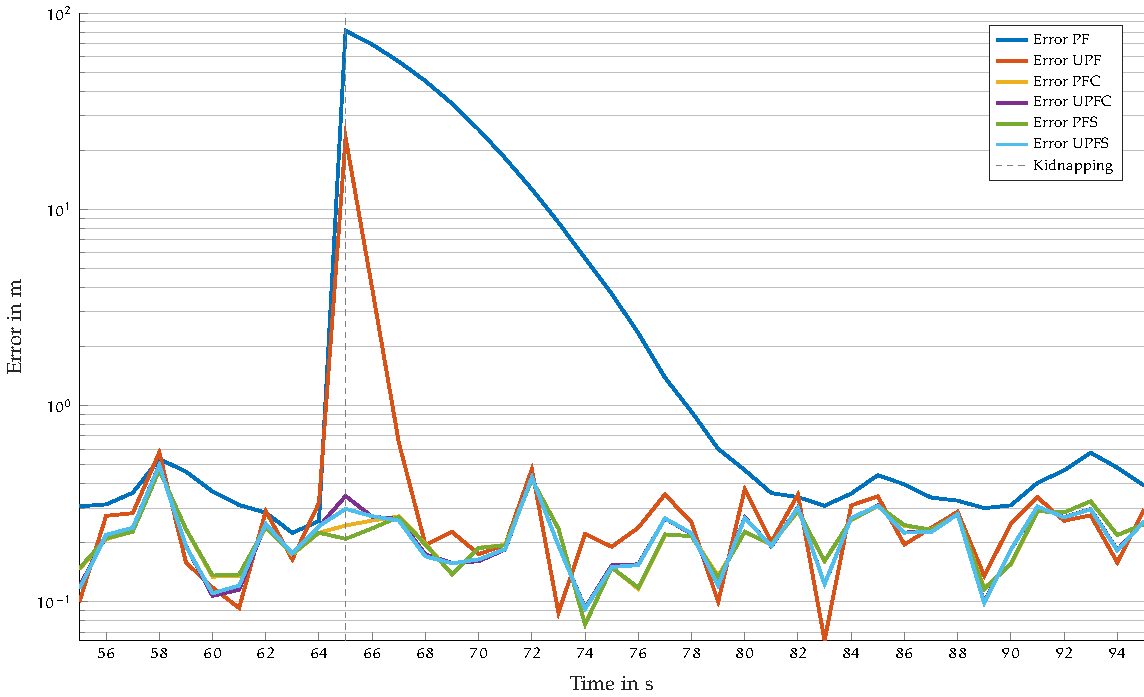
\includegraphics[height=1.0\textwidth]{Tikz/Results/2018-09-03-13-54-12-results-figure-6.tikz}}			
	\caption[First 30 seconds of the mean estimation error over time after kidnapping in Scenario 3. \texttt{PF}, \texttt{PFC}, \texttt{PFS}: 10000 particles. \texttt{UPF}, \texttt{UPFC}, \texttt{UPFS}: 100 particles.]
	{First 30 seconds of the mean estimation error over time after kidnapping in Scenario 3 (logarithmic scale). \texttt{PF}, \texttt{PFC}, \texttt{PFS}: 10000 particles. \texttt{UPF}, \texttt{UPFC}, \texttt{UPFS}: 100 particles.}
	\label{fig:2018-09-03-13-54-12-results-figure-6}			
\end{figure}



\section{Discussion}\label{sec:discussion}

Given the results presented in the previous section, we will now discuss them in detail, first comparing the new against the respective conventional localisation algorithms in the following two sections and then comparing the bootstrap particle filters against the unscented particle filters in Section \ref{sec:unscentedvspf}. Finally, we will discuss the differences between the results of the filters using the \texttt{HC4} contractor and those using \texttt{SIVIA}.

\subsection[Bootstrap Filters]{Constraint vs. Unconstraint Bootstrap Filters}

First, the constraint bootstrap filters (\texttt{PFC}, \texttt{PFS}) and the unconstrained bootstrap filter (\texttt{PF}) are contrasted in the respective localisation scenarios. Comparing the median estimation error of the bootstrap particle filter with \texttt{HC4} contractor and with \texttt{SIVIA}, respectively, against the median error of the conventional bootstrap filter, one can see that both new filter algorithms consistently outperform the conventional one in each of the experiments, while the median error of the \texttt{PFS} is smaller or equal to that of the \texttt{PFC} (cf. box plots in Figures \ref{fig:2018-09-30-12-09-00-results-figure-1}, \ref{fig:2018-10-04-15-13-55-results-figure-1}, \ref{fig:2018-09-24-11-26-33-results-figure-1}, \ref{fig:2018-09-21-21-56-07-results-figure-1}, \ref{fig:2018-08-30-19-17-11-results-figure-1}, \ref{fig:2018-09-03-13-54-12-results-figure-1}). However, the difference in median errors is less pronounced for an increased number of landmarks, as can be seen in the box plots for the scenarios with four and nine landmarks in Figures \ref{fig:2018-09-24-11-26-33-results-figure-1}, \ref{fig:2018-09-21-21-56-07-results-figure-1}, \ref{fig:2018-08-30-19-17-11-results-figure-1}, \ref{fig:2018-09-03-13-54-12-results-figure-1}. In these scenarios, in turn, the initial estimation error and the error right after kidnapping is reduced significantly (cf. mean error plots in Figures \ref{fig:2018-09-24-11-26-33-results-figure-7}, \ref{fig:2018-09-21-21-56-07-results-figure-8}, \ref{fig:2018-08-30-19-17-11-results-figure-6}, \ref{fig:2018-09-03-13-54-12-results-figure-6}). It should be noted that in these figures the higher error of the conventional bootstrap filter after convergence is due to different tuning of the filters, which takes into account the confined search space in case of the hybrid filter algorithms.

\begin{table*}\centering
\ra{1.3}
\begin{tabular}{@{}lrrrrrrr@{}}\toprule
& \multicolumn{3}{c}{Wake-up r. p.} & \phantom{a} & \multicolumn{3}{c}{Kidnapped r. p.} \\ 
\cmidrule{2-4} \cmidrule{6-8}
 & \multicolumn{1}{c}{\texttt{PF}} & \multicolumn{1}{c}{\texttt{PFC}} & \multicolumn{1}{c}{\texttt{PFS}} & & \multicolumn{1}{c}{\texttt{PF}} & \multicolumn{1}{c}{\texttt{PFC}} & \multicolumn{1}{c}{\texttt{PFS}} \\
\midrule 
Median error in m & $18.6$ & $9.9$ & $5.6$ & & $79.6$ & $20.0$ & $9.8$ \\              
Improvement in \%  & -- & $47$ & $70$ & & -- & $75$ & $88$ \\ 
\bottomrule
\end{tabular}
\caption{Median errors for the bootstrap filters in Scenario 1.}
\label{tab:median_scenario1}
\end{table*}

%\subsubsection{Scenario 1}

In Scenario 1, with a median error of 9.9 metres for the \texttt{PFC} and 18.6 metres for the conventional bootstrap filter, this represents an improvement of 47 percent. The \texttt{PFS} achieves a median error of less than 5.6 metres, which makes up for an improvement of 70 percent (cf. box plot in Figure \ref{fig:2018-09-30-12-09-00-results-figure-1}). When kidnapping the robot in Scenario 1, the respective improvements are 75 percent for the \texttt{PFC} and 88 percent for the \texttt{PFS}, given median errors of 79.6 metres (\texttt{PF}), 20 metres (\texttt{PFC}), and 9.8 metres (\texttt{PFS}), which can also be seen in the box plot in Figure \ref{fig:2018-10-04-15-13-55-results-figure-1}. The median errors and the respective improvement in percent is contrasted in Table \ref{tab:median_scenario1}.



%\subsubsection{Scenario 2}

In the presence of four landmarks, the mean initial estimation error is reduced by 13 percent for the \texttt{PFC} and by 91 percent for the \texttt{PFS}, given the mean initial errors of 5.8 metres (\texttt{PF}), 5.1 metres (\texttt{PFC}), and 0.5 metres (\texttt{PFS}), which can be seen in the mean error plot in Figure \ref{fig:2018-09-24-11-26-33-results-figure-7}. The major difference in error between the \texttt{PFC} and the \texttt{PFS} will be discussed in Section \ref{contrvssivia}. The mean first error after kidnapping is reduced by 94 percent for the \texttt{PFC} and by 99 percent for the \texttt{PFS}, given the mean initial errors of 80.8 metres (\texttt{PF}), 4.7 metres (\texttt{PFC}), and 0.6 metres (\texttt{PFS}), which are depicted in the mean error plot in Figures \ref{fig:2018-09-21-21-56-07-results-figure-8}. The mean initial errors and the respective improvement in percent are contrasted in Table \ref{tab:mean_scenario2}. The lower initial errors and the faster convergence of the two hybrid bootstrap filters are also reflected in the number of outliers in the box plots depicted in Figures \ref{fig:2018-09-24-11-26-33-results-figure-1} and \ref{fig:2018-09-21-21-56-07-results-figure-1}. 

\begin{table*}\centering
\ra{1.3}
\begin{tabular}{@{}lrrrrrrr@{}}\toprule
& \multicolumn{3}{c}{Wake-up r. p.} & \phantom{a} & \multicolumn{3}{c}{Kidnapped r. p.} \\ 
\cmidrule{2-4} \cmidrule{6-8}
 & \multicolumn{1}{c}{\texttt{PF}} & \multicolumn{1}{c}{\texttt{PFC}} & \multicolumn{1}{c}{\texttt{PFS}} & & \multicolumn{1}{c}{\texttt{PF}} & \multicolumn{1}{c}{\texttt{PFC}} & \multicolumn{1}{c}{\texttt{PFS}} \\
\midrule 
Mean initial error in m & $5.8$ & $5.1$ & $0.5$ & & $80.8$ & $4.7$ & $0.6$ \\              
Improvement in \%  & -- & $13$ & $91$ & & -- & $94$ & $99$ \\ 
\bottomrule
\end{tabular}
\caption{Mean initial errors and errors after kidnapping for the bootstrap filters in Scenario 2.}
\label{tab:mean_scenario2}
\end{table*}


%\subsubsection{Scenario 3}

In Scenario 3, the error of the \texttt{PFC} and \texttt{PFS} is smaller than 60 centimetres throughout the whole estimation process. That is, both hybrid bootstrap filters converge instantly, as can be seen in the mean error plots in Figure \ref{fig:2018-08-30-19-17-11-results-figure-6} without kidnapping and in Figure \ref{fig:2018-09-03-13-54-12-results-figure-6} with kidnapping. In contrast, due to the high initial errors, the conventional bootstrap filter only achieves an upper error bound of 16.8 metres without kidnapping (cf. box plots in Figures \ref{fig:2018-08-30-19-17-11-results-figure-1}) and of 86.7 metres with kidnapping (cf. box plot in Figures \ref{fig:2018-09-03-13-54-12-results-figure-1}). The major improvement is due to the bounded-error estimation that is carried out when performing global localisation in the beginning and the reliable detection of kidnapping, which restarts the global localisation process likewise. The individual mean initial errors and the respective improvement in percent are contrasted in Table \ref{tab:mean_scenario3} (cf. also mean error plots in Figures \ref{fig:2018-08-30-19-17-11-results-figure-6}, \ref{fig:2018-09-03-13-54-12-results-figure-6}).


\begin{table*}\centering
\ra{1.3}
\begin{tabular}{@{}lrrrrrrr@{}}\toprule
& \multicolumn{3}{c}{Wake-up r. p.} & \phantom{a} & \multicolumn{3}{c}{Kidnapped r. p.} \\ 
\cmidrule{2-4} \cmidrule{6-8}
 & \multicolumn{1}{c}{\texttt{PF}} & \multicolumn{1}{c}{\texttt{PFC}} & \multicolumn{1}{c}{\texttt{PFS}} & & \multicolumn{1}{c}{\texttt{PF}} & \multicolumn{1}{c}{\texttt{PFC}} & \multicolumn{1}{c}{\texttt{PFS}} \\
\midrule 
Mean initial error in m & $6.5$ & $0.36$ & $0.36$ & & $81.2$ & $0.24$ & $0.21$ \\              
Improvement in \%  & -- & $94$ & $94$ & & -- & $99$ & $99$ \\ 
\bottomrule
\end{tabular}
\caption{Mean initial errors and errors after kidnapping for the bootstrap filters in Scenario 3.}
\label{tab:mean_scenario3}
\end{table*}


\subsection[Unscented Particle Filters]{Constraint vs. Unconstraint Unscented Particle Filters}

In this section, the constraint unscented particle filters (\texttt{UPFC}, \texttt{UPFS}) are compared against the unconstrained unscented particle filter (\texttt{UPF}). With two available landmarks, the median estimation error of the constraint unscented particle filters is up to 30 metres smaller than that of the conventional unscented particle filters (cf. box plot in Figure \ref{fig:2018-09-30-12-09-00-results-figure-1}), while both \texttt{UPFC} and \texttt{UPFS} have similar initial estimation errors before they slightly drift apart, as can be seen in Figure \ref{fig:2018-09-30-12-09-00-results-figure-5}. This can be explained by the probabilistic nature of the filters. Looking at the results of the individual runs in the GitHub repository \cite{codeGithub}, one can observe the high error variance of the \texttt{UPFS}.

When four or nine landmarks are available, the median errors of both the \texttt{UPFC} and the \texttt{UPFS} are similar to that of the \texttt{UPF} (cf. box plots in Figures \ref{fig:2018-09-24-11-26-33-results-figure-1}, \ref{fig:2018-09-21-21-56-07-results-figure-1}, \ref{fig:2018-08-30-19-17-11-results-figure-1}, \ref{fig:2018-09-03-13-54-12-results-figure-1}). However, in these scenarios the mean initial estimation error as well as the mean first error after kidnapping is significantly reduced by the bounded-error state estimation (cf. mean error plots in Figures \ref{fig:2018-09-24-11-26-33-results-figure-7}, \ref{fig:2018-09-21-21-56-07-results-figure-8}, \ref{fig:2018-08-30-19-17-11-results-figure-6}, \ref{fig:2018-09-03-13-54-12-results-figure-6}). Both the lower initial errors and the faster convergence of the two hybrid unscented particle filters is also reflected in the number of outliers in the box plots depicted in Figures \ref{fig:2018-09-24-11-26-33-results-figure-1}, \ref{fig:2018-09-21-21-56-07-results-figure-1}, \ref{fig:2018-08-30-19-17-11-results-figure-1}, \ref{fig:2018-09-03-13-54-12-results-figure-1}.


In the presence of four landmarks, the mean initial estimation error is reduced by 64 percent for the \texttt{UPFC} and by 92 percent for the \texttt{UPFS}, given the mean initial errors of 6.4 metres (\texttt{UPF}), 2.3 metres (\texttt{UPFC}), and 0.5 metres (\texttt{UPFS}), which can be seen in the mean error plot in Figure \ref{fig:2018-09-24-11-26-33-results-figure-7}. The mean first error after kidnapping is reduced by 76 percent for the \texttt{UPFC} and by 98 percent for the \texttt{UPFS}, given the mean initial errors of 49.4 metres (\texttt{UPF}), 12.1 metres (\texttt{UPFC}), and 0.7 metres (\texttt{UPFS}), which are depicted in the mean error plot in Figures \ref{fig:2018-09-21-21-56-07-results-figure-8}. The mean initial errors and the respective improvement in percent are contrasted in Table \ref{tab:mean_scenario2_u}.

\begin{table*}\centering
\ra{1.3}
\begin{tabular}{@{}lrrrrrrr@{}}\toprule
& \multicolumn{3}{c}{Wake-up r. p.} & \phantom{a} & \multicolumn{3}{c}{Kidnapped r. p.} \\ 
\cmidrule{2-4} \cmidrule{6-8}
 & \multicolumn{1}{c}{\texttt{UPF}} & \multicolumn{1}{c}{\texttt{UPFC}} & \multicolumn{1}{c}{\texttt{UPFS}} & & \multicolumn{1}{c}{\texttt{UPF}} & \multicolumn{1}{c}{\texttt{UPFC}} & \multicolumn{1}{c}{\texttt{UPFS}} \\
\midrule 
Mean initial error in m & $6.4$ & $2.3$ & $0.5$ & & $49.4$ & $12.1$ & $0.7$ \\              
Improvement in \%  & -- & $64$ & $92$ & & -- & $76$ & $98$ \\ 
\bottomrule
\end{tabular}
\caption{Mean initial errors and errors after kidnapping for the unscented particle filters in Scenario 2.}
\label{tab:mean_scenario2_u}
\end{table*}

In Scenario 3, the error of the \texttt{UPFC} and \texttt{UPFS} is always smaller than 70\,cm (Figures \ref{fig:2018-08-30-19-17-11-results-figure-1}, \ref{fig:2018-09-03-13-54-12-results-figure-1}), whereas the upper error bound remains high for the conventional unscented particle filter at 23.3 metres with kidnapping and 17.6 metres without kidnapping. Again, this is due to the reduction in the size of the initial search space achieved by the bounded-error estimation. The mean initial errors and the respective improvement in percent are contrasted in Table \ref{tab:mean_scenario3_u}.

%Given very ambiguous measurements, that is only two landmarks are available, the constraint unscented particle filters generally deliver only slightly lower mean errors and in some cases even higher mean errors, as can be seen in Figures \ref{fig:2018-09-29-14-05-04-results-figure-5}, \ref{fig:2018-09-29-14-05-04-results-figure-7}, \ref{fig:2018-10-04-15-13-55-results-figure-6}, \ref{fig:2018-09-30-01-28-57-results-figure-6}, and \ref{fig:2018-09-28-21-07-55-results-figure-6}. This confirms the theory in that a relatively large box obtained on the basis of only two landmarks should not influence the performance of the unscented particle filter very much. In fact, it seems that the influence of the bounded-error state estimate is negligible as the individual results are very similar for the \texttt{UPF}, the \texttt{UPFC}, and the \texttt{UPFS}. Presumably, they would tend to the same values when the number of runs of the experiments is increased further. The shortcomings of the unscented particle filters in scenarios with little information will be discussed further in the following section.

\begin{table*}\centering
\ra{1.3}
\begin{tabular}{@{}lrrrrrrr@{}}\toprule
& \multicolumn{3}{c}{Wake-up r. p.} & \phantom{a} & \multicolumn{3}{c}{Kidnapped r. p.} \\ 
\cmidrule{2-4} \cmidrule{6-8}
 & \multicolumn{1}{c}{\texttt{UPF}} & \multicolumn{1}{c}{\texttt{UPFC}} & \multicolumn{1}{c}{\texttt{UPFS}} & & \multicolumn{1}{c}{\texttt{UPF}} & \multicolumn{1}{c}{\texttt{UPFC}} & \multicolumn{1}{c}{\texttt{UPFS}} \\
\midrule 
Mean initial error in m & $3.7$ & $0.4$ & $0.4$ & & $23.2$ & $0.3$ & $0.3$ \\              
Improvement in \%  & -- & $89$ & $89$ & & -- & $99$ & $99$ \\ 
\bottomrule
\end{tabular}
\caption{Mean initial errors and errors after kidnapping for the unscented particle filters in Scenario 3.}
\label{tab:mean_scenario3_u}
\end{table*}


\subsection[Bootstrap vs. Unscented Particle Filters]{Bootstrap Filters vs. Unscented Particle Filters}\label{sec:unscentedvspf}

When comparing the bootstrap particle filters (\texttt{PF}, \texttt{PFC}, \texttt{PFS}) against the unscented
particle filters (\texttt{UPF}, \texttt{UPFC}, \texttt{UPFS}), the results confirm the theory. If the likelihood is very peaked, given very accurate measurements and an unambiguous scenario like Scenario 2 or 3, the unscented particle filter and its constrained counterparts make better use of the existing particles by incorporating the latest measurement into the proposal distribution. As can be seen in the mean error plots in Figures \ref{fig:2018-09-24-11-26-33-results-figure-7}, \ref{fig:2018-09-21-21-56-07-results-figure-8}, \ref{fig:2018-08-30-19-17-11-results-figure-6}, \ref{fig:2018-09-03-13-54-12-results-figure-6}, the mean estimation error of the unscented particle filters decreases faster than that of the bootstrap particle filters, since particles are actively moved towards the peak of the likelihood function. Especially when using a contractor, whose resulting box in Scenario 2 has still a considerable volume, the unscented particle filter can improve the estimation accuracy in the beginning of the global localisation process. Figure \ref{fig:2018-09-24-11-26-33-results-figure-7} shows how the mean initial error is 2.3 metres for the \texttt{UPFC} in contrast to 5 metres for the \texttt{PFC}, since the \texttt{UPFC} incorporates the first measurement when propagating the initial particle distribution. In addition to that, the \texttt{UPFC} increases the speed of convergence. The mean estimation error falls below 1 metre in 7 seconds for the \texttt{PFC}, whereas the \texttt{UPFC} only takes 1 second.

When nine landmarks are visible, the constrained unscented particle filters do not noticeably improve the estimation accuracy when compared to the constrained bootstrap filters. The mean estimation errors of the \texttt{PFC}, \texttt{UPFC}, \texttt{PFS}, and \texttt{UPFS} are consistently below 70 centimetres, as can be seen in the box plots in Figures \ref{fig:2018-08-30-19-17-11-results-figure-1}, \ref{fig:2018-09-03-13-54-12-results-figure-1} and the mean error plots in Figures \ref{fig:2018-08-30-19-17-11-results-figure-4}, \ref{fig:2018-09-03-13-54-12-results-figure-4}). This can be explained by the very narrow box that confines the initial set of uniformly spread particles. Given such narrow region, particles are already close to the peak of the likelihood function and the overlap of the proposal distribution and the posterior distribution is already large, due to the bounded-error estimation. The lower bound in the median error of approximately 20 centimetres is to be explained by the finitely accurate measurements. It may be possible to lower it by more accurate measurements, but using an increased number of particles or more elaborate filtering techniques will presumably not improve the estimation accuracy further, which for many practical applications appears to be sufficient.
  

%When looking at the initial mean error and at the mean error shortly after kidnapping of the \texttt{PFC} and \texttt{UPFC} in Figures \ref{fig:2018-09-24-11-26-33-results-figure-7}, \ref{fig:2018-09-23-20-54-13-results-figure-7}, \ref{fig:2018-09-21-16-00-07-results-figure-7}, \ref{fig:2018-09-21-21-56-07-results-figure-8}, \ref{fig:2018-09-23-12-42-11-results-figure-8}, and \ref{fig:2018-09-21-10-11-38-results-figure-8}, a major improvement can also be seen here. Given a medium-sized initial box obtained by the contractor, when compared to the results in Scenarios 1 and 3, the \texttt{UPFC} brings down the error a lot faster than the \texttt{PFC} does. 



When only two landmarks are available, that is the measurements are ambiguous and a large region of the state space has a high observation likelihood, the three unscented particle filters fail to converge quickly (cf. mean error plots in Figures \ref{fig:2018-09-30-12-09-00-results-figure-5}, \ref{fig:2018-10-04-15-13-55-results-figure-6}). As opposed to the bootstrap particle filters, which merely move the particles according to the system model, the unscented particle filters actively move particles to regions of high likelihood. However, if the likelihood is not concentrated in certain regions of the search space, this movement may in fact be counterproductive. In those unambiguous scenarios, the bootstrap filter indeed benefits from the fact that it only moves the particles according to the system model, so that physical movement of the robot adds information when the measurements themselves do not provide sufficient information to unambiguously localise the robot. In other words, when one does not know precisely enough where to move particles to, regarding the observations, one should merely move according to the system model.

In summary, the more information is available to move particles to regions of high likelihood, the more pronounced the improvement of an unscented particle filter will be. However, with a box estimate that has sufficiently small volume already and with an accurate system model, the effect may be insignificant. 


\begin{figure}
	\centering
	\setlength\figureheight{0.7\textwidth} 	
	\setlength\figurewidth{0.9\textwidth}		
	\tikzsetnextfilename{largeSivia}		
	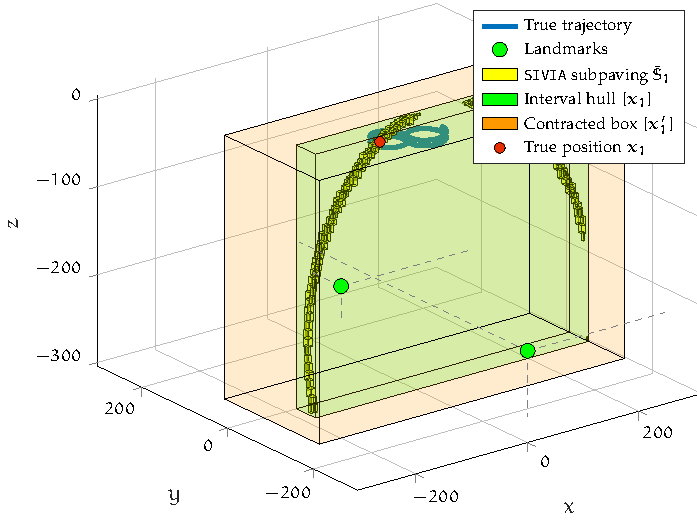
\includegraphics[width=\textwidth]{Tikz/largeSivia.tikz}	
	\caption[Comparison of a \texttt{SIVIA} subpaving and a contracted box in Scenario 1.]{Comparison of the \texttt{SIVIA} subpaving $\bar{\mathbb{S}}_1$ its interval hull $[\bm{x}_1]$ and the contracted box $[\bm{x}_1']$ in Scenario 1 with two landmarks.}			
	\label{fig:largeSivia}			
\end{figure}

\begin{figure}
	\centering
	\setlength\figureheight{0.7\textwidth} 	
	\setlength\figurewidth{0.9\textwidth}		
	\tikzsetnextfilename{smallSivia}		
	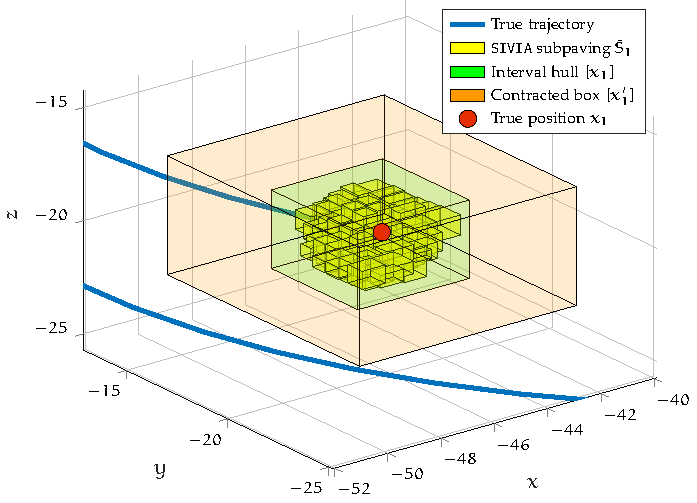
\includegraphics[width=\textwidth]{Tikz/smallSivia.tikz}	
	\caption[Comparison of a \texttt{SIVIA} subpaving and a contracted box in Scenario 3.]{Comparison of the \texttt{SIVIA} subpaving $\bar{\mathbb{S}}_1$ its interval hull $[\bm{x}_1]$ and the contracted box $[\bm{x}_1']$ in Scenario 3 with nine landmarks.}			
	\label{fig:smallSivia}			
\end{figure}

\subsection{\texttt{HC4} Contractor vs. \texttt{SIVIA}}\label{contrvssivia}

The \texttt{SIVIA} algorithm may find a better approximation of the solution set described by the constraints than the contractor, especially when its shape strongly deviates from that of a cuboid in three-dimensions or an $n_{\bm{x}}$-orthotope for higher dimensional state spaces. However, since we use the hull of the \texttt{SIVIA} subpaving as a confinement for the spreading of particles, in practice the difference may be minor, especially for an increased number of  landmarks. This is depicted in Figures \ref{fig:largeSivia} and \ref{fig:smallSivia}, which compare the interval hull $[\bm{x}_1]$ of the \texttt{SIVIA} subpaving with the contracted box, here denoted with $[\bm{x}_1']$, both based on the first measurement in Scenario 1 and 3, respectively. The results show that the more information in terms of landmarks is available, the less marked the difference in volume and therefore the impact on the increase in estimation accuracy will be.

The box plots in Figures \ref{fig:2018-08-30-19-17-11-results-figure-1} and \ref{fig:2018-09-03-13-54-12-results-figure-1} show very similar errors for both the contractor and \texttt{SIVIA} in Scenario 3, while the box plots in Figure \ref{fig:2018-09-24-11-26-33-results-figure-1} and \ref{fig:2018-09-21-21-56-07-results-figure-1} indicate a difference in the error distribution for the contractor and \texttt{SIVIA} in Scenario 2. In particular, the number of outliers is reduced, as the initial errors are lower and therefore convergence  takes place more rapidly. The volume of the contracted box is usually larger than that of the hull, but relating the difference in size to the vastly larger computational demands of \texttt{SIVIA}, for a practical application the difference may be insignificant and remains to be tested experimentally in a specific localisation scenario. 






